\documentclass[12pt,a4paper,twoside]{scrartcl}
\usepackage[ngerman,english]{babel}
\usepackage[T1]{fontenc}
\usepackage{lmodern}
\usepackage[utf8]{inputenc}
\usepackage[tmargin=22mm,bmargin=22mm,lmargin=20mm,rmargin=20mm]{geometry}
\usepackage{latexsym,amsmath,amssymb,mathtools,textcomp}
\usepackage{parskip}
\usepackage{amsthm}
\usepackage{bbm}
\usepackage{mathtools}
\usepackage{indentfirst}

\begingroup
\makeatletter
\@for\theoremstyle:=definition,remark,plain\do{%
  \expandafter\g@addto@macro\csname th@\theoremstyle\endcsname{%
    \addtolength\thm@preskip\parskip
  }%
}
\endgroup

\newtheorem{theorem}{Theorem}[section]
\newtheorem{definition}[theorem]{Definition}
\newtheorem{lemma}[theorem]{Lemma}

\numberwithin{equation}{section}
\DeclareOldFontCommand{\bf}{\normalfont\bfseries}{\mathbf}

\usepackage{graphicx}
\graphicspath{{images/}}
\usepackage{array,multirow}
\usepackage{enumitem}
\setlist[enumerate]{topsep=0pt}
\setlist[itemize]{topsep=0pt}
\setlist[description]{font=\normalfont,topsep=0pt}
\setlist[enumerate,1]{label=(\roman*)}

\usepackage{tikz}
\usetikzlibrary{calc}
\usepackage{fancyhdr}
\fancypagestyle{plain}{
  \setlength\footskip{32pt}
  \fancyhead{}
  \fancyfoot{}
  \fancyfoot[LE,RO]{\normalsize\thepage}
  \renewcommand{\headrulewidth}{0pt}
  \renewcommand{\footrulewidth}{0pt}
}

\usepackage{ctable}
\fancypagestyle{normal}{
  \setlength{\headheight}{20pt}
  \setlength\footskip{32pt}
  \fancyhead{}
  \fancyhead[LE]{\normalsize\textsc{\nouppercase{\leftmark}}}
  \fancyhead[RO]{\normalsize\textsc{\nouppercase{\rightmark}}}
  \fancyfoot{}
  \fancyfoot[LE,RO]{\normalsize\thepage}
  \renewcommand{\headrulewidth}{0.4pt}
  \renewcommand{\footrulewidth}{0pt}
}

\usepackage{color}
\usepackage[pagebackref]{hyperref}
\usepackage[all]{hypcap}
\usepackage{cleveref}

\hypersetup{
  pdftitle={Creating and Evaluating Stochastic Regression Models on the Basis of Heterogeneous Sensor Networks}, %TODO
  pdfauthor={Stanislav Arnaudov}, %TODO
  pdfsubject={machine learning, probabilistic forecast, bayesian neural networks, mixture density networks, proper scoring rules, fea2ture importance}, %TODO
  colorlinks=true,
  pdfborder={0 0 0},
  bookmarksopen=true,
  bookmarksopenlevel=1,
  bookmarksnumbered=true,
  linkcolor=blue!60!black,
  % linkcolor=black,
  citecolor=blue!60!black,
  urlcolor=blue!60!black,
  filecolor=green!60!black,
  pdfpagemode=UseNone,
  unicode=true,
}

\renewcommand*{\backreflastsep}{, }
\renewcommand*{\backreftwosep}{, }
\renewcommand*{\backref}[1]{}
\renewcommand*{\backrefalt}[4]{%
  \ifcase #1 %
  No citations.% use \relax if you do not want the "No citations" message %TODO
  \or
  (Page #2).%
  \else
  (Pages #2).%
  \fi%
}
\usepackage{import}

\newcommand{\reflst}[1]{\hyperref[#1]{Listing~\ref*{#1}}}
\newcommand{\refthm}[1]{\hyperref[#1]{Theorem~\ref*{#1}}}
\newcommand{\refdef}[1]{\hyperref[#1]{Definition~\ref*{#1}}}

\newcommand{\reffig}[1]{\hyperref[#1]{Figure \ref*{#1}}}
\newcommand{\refsec}[1]{\hyperref[#1]{Section \ref*{#1}}}
\newcommand{\reftab}[1]{\hyperref[#1]{Table \ref*{#1}}}
\renewcommand*{\refeq}[1]{\hyperref[#1]{Equation \ref*{#1}}}





% Package for inserting pseudo codes in the document.
\usepackage[ruled,vlined,linesnumbered,norelsize]{algorithm2e}
\DontPrintSemicolon
\def\NlSty#1{\textnormal{\fontsize{8}{10}\selectfont{}#1}}
\SetKwSty{texttt}
\SetCommentSty{emph}
\def\listalgorithmcfname{List of Algorithms}
\def\algorithmautorefname{Algorithm}
\let\chapter=\section % resolve a problem with algorithm2


\begin{document}
\boldmath
% \frenchspacing
\nonfrenchspacing

\pagestyle{empty}
\pagenumbering{alph}


\setlength{\parindent}{4em}
\setlength{\parskip}{1em}

% title page
\begin{titlepage}

  \begin{center}\large

    {\flushleft
\includegraphics[height=17mm, width=45mm]{kit_logo_en.pdf} \hfill}
    
\includegraphics[height=15mm, width=45mm]{group_logo.pdf}\quad\null

    \vspace*{1cm}

    Bachelor's Thesis
    \vspace*{1cm}

    {\bf\huge Creating and Evaluating  Stochastic Regression Models on the Basis of Heterogeneous Sensor Networks. \par} %TODO

    \vfill

    by\\
    \vspace*{3mm}
    {\huge{Stanislav Arnaudov}}
    

    \vspace*{10mm}
    Chair of Pervasive Computing Systems/TECO,\\
    Institute of Telematics\\
    Department of Informatics\\
    \vspace*{20mm}

    Handover Date: 31.09.2018

    \vspace*{20mm}

    
    
    \begin{tabular}{rl}
      Supervisors: &Dr. Johannes Riesterer\(^1\) \\
                   &Dr. Sebastian Lerch\(^{2,3}\)     \\
    \end{tabular}
    
    \vspace*{10mm}


    \(^1\)Chair for Pervasive Computing Systems / TECO, Institute of Telematics, Karlsruhe Institute of Technology\\
    \(^2\)Institute for Stochastics, Karlsruhe Institute of Technology\\
    \(^3\)Heidelberg Institute for Theoretical Studies

    \vspace*{12mm}
  \end{center}

\end{titlepage}


\selectlanguage{english}

\centerline{\bf Statement of Authorship}
\vfill

I hereby declare that I am the sole author of this bachelor thesis  and that I have not used any sources other than those listed in the bibliography and identified as references. I further declare that I have not submitted this thesis at any other institution in order to obtain a degree.

\vfill
\noindent

\selectlanguage{ngerman}
\vfill
Hiermit versichere ich, dass ich diese Arbeit selbständig verfasst und keine anderen, als die angegebenen Quellen und Hilfsmittel benutzt, die wörtlich oder inhaltlich übernommenen Stellen als solche kenntlich gemacht und die Satzung des Karlsruher Instituts für Technologie zur Sicherung guter wissenschaftlicher Praxis in der jeweils gültigen Fassung beachtet habe.
\vfill
\noindent
Karlsruhe, 31.09.2018
\hrule


\vspace*{5cm}

\clearpage

%%%%%%%%%%%%%%%%%%%%%%%%%%%%%%%%%%%%%%%%%%%%%%%%%%%%%%%%%%%%%%%%%%%%%% 

\vspace*{0pt}\vfill

\selectlanguage{english}

\begin{abstract}
  \centerline{\bf Abstract}
  This thesis aims to better understand Bayesian machine learning models and their practical use on real world data. We examine two models that incorporate uncertainty in their predictions - Bayesian Neural Networks and Mixture Density Networks. The used data comes from air-pollution sensors. The quality of 3 of the sensors is known to be high but for the rest of them the quality of measurement is unknown. We aim to build a model that can predict the air pollution at some sensor at a given time. Consideration of the uncertainty in the predicted value is crucial as it allows the precise evaluation of the generated models. We compare the models through evaluation with proper scoring rules. As the quality of the majority of sensors is from unknown quality we try to find out which of the sensors are most relevant for a better prediction through a feature importance technique. We leverage the capabilities of Tensorflow, Edward and GPFlow machine learning libraries in order to build probabilistic regression models that can be further evaluated.
\end{abstract}

\vfill\vfill\vfill
\clearpage

%%%%%%%%%%%%%%%%%%%%%%%%%%%%%%%%%%%%%%%%%%%%%%%%%%%%%%%%%%%%%%%%%%%%%% 
\selectlanguage{english}
\pagestyle{plain}
\pagenumbering{roman}

% markiere sections im Seitenkopf links und subsections rechts
\renewcommand\sectionmark[1]{\markboth{\thesection\quad\MakeUppercase{#1}}{\thesection\quad\MakeUppercase{#1}}}
\renewcommand\subsectionmark[1]{\markright{\thesubsection\quad\MakeUppercase{#1}}}

\tableofcontents
\clearpage
%%%%%%%%%%%%%%%%%%%%%%%%%%%%%%%%%%%%%%%%%%%%%%%%%%%%%%%%%%%%%%%%%%%%%% 
\listoffigures
\clearpage



\pagestyle{normal}
\pagenumbering{arabic}
% here comes  the text!

\section{Introduction}
\label{sec:intoduction}
\subsection{Motivation}
\label{sec:motivation}

There are a lot of cases where a network of sensors is used to measure a certain quantity over time in different places. Some of the measurements can have better \emph{quality} than other as not all sensors are created equal. With quality we mean the reliability that the measured value indeed reflects the reality. The difference in the quality of the sensors  makes the measured data \emph{heterogeneous} and brings certain difficulties in the modeling process. For a machine learning application only some of the data maybe relevant for building a reliable predictive model. One of our goals is to asses which part of the input is useful data and to what extend.

From another point of view we can also set another goal. We consider the case where only a few of the sensors are known to produce reliable measurements. In this sense we try to expand a network of \emph{homogeneous} and high reliability sensors with sensors of unknown quality and thus making the network heterogeneous. In this case we increase the spatial resolution of the network and thus we bring the possibility to make more accurate predictions on the basis of data coming from the whole network. On the other hand, heterogeneity in quality of the different sources in the network introduces uncertainty in the measurements. It thus becomes necessary to build appropriate model that predicts the measured values from given sensor but also respects the inherent uncertainty in the data and also models it properly.

To concertize the problem - we use air pollution data from a network of sensors around Stuttgart. The Landesanstalt für Umwelt, Messungen und Naturschutz Baden-Württemberg (\href{https://www.lubw.baden-wuerttemberg.de/startseite}{LU-BW}) has provided data from 3 high quality air pollution sensors. The other part of the data is from \emph{DIY} (\emph{Do it yourself}) sensors that provide their measurements publicly under \href{https://luftdaten.info/}{luftdaten.info}. Those are the unreliable parts of the  network as described in the previous paragraph. We can make no statements about the quality of the data coming form the DIY sensors. We do not know how are they calibrated and the sensors are deployed from anonymous builders. Furthermore the sensors are cheap. All of this effectively means that we have unreliable features in our input data. We aim to find out which of the features (and with that which of the sensors) are ``better'' than the others. This is done through a \emph{feature importance} technique described in \refsec{sec:feature-importance}. We also investigate whether or not we can predict the air pollution values measured by one of the LUBW-sensors based on the combined data coming from all other  sensors. If reliable predictions are possible, this would suggest that one can theoretically use the cheap network of sensors as an substitute for the few high quality sensors. \reffig{fig:general} shows the general overview of the system we want to develop.



\begin{center}
  \begin{figure}[htbp]
    \label{fig:general}
    \centering
    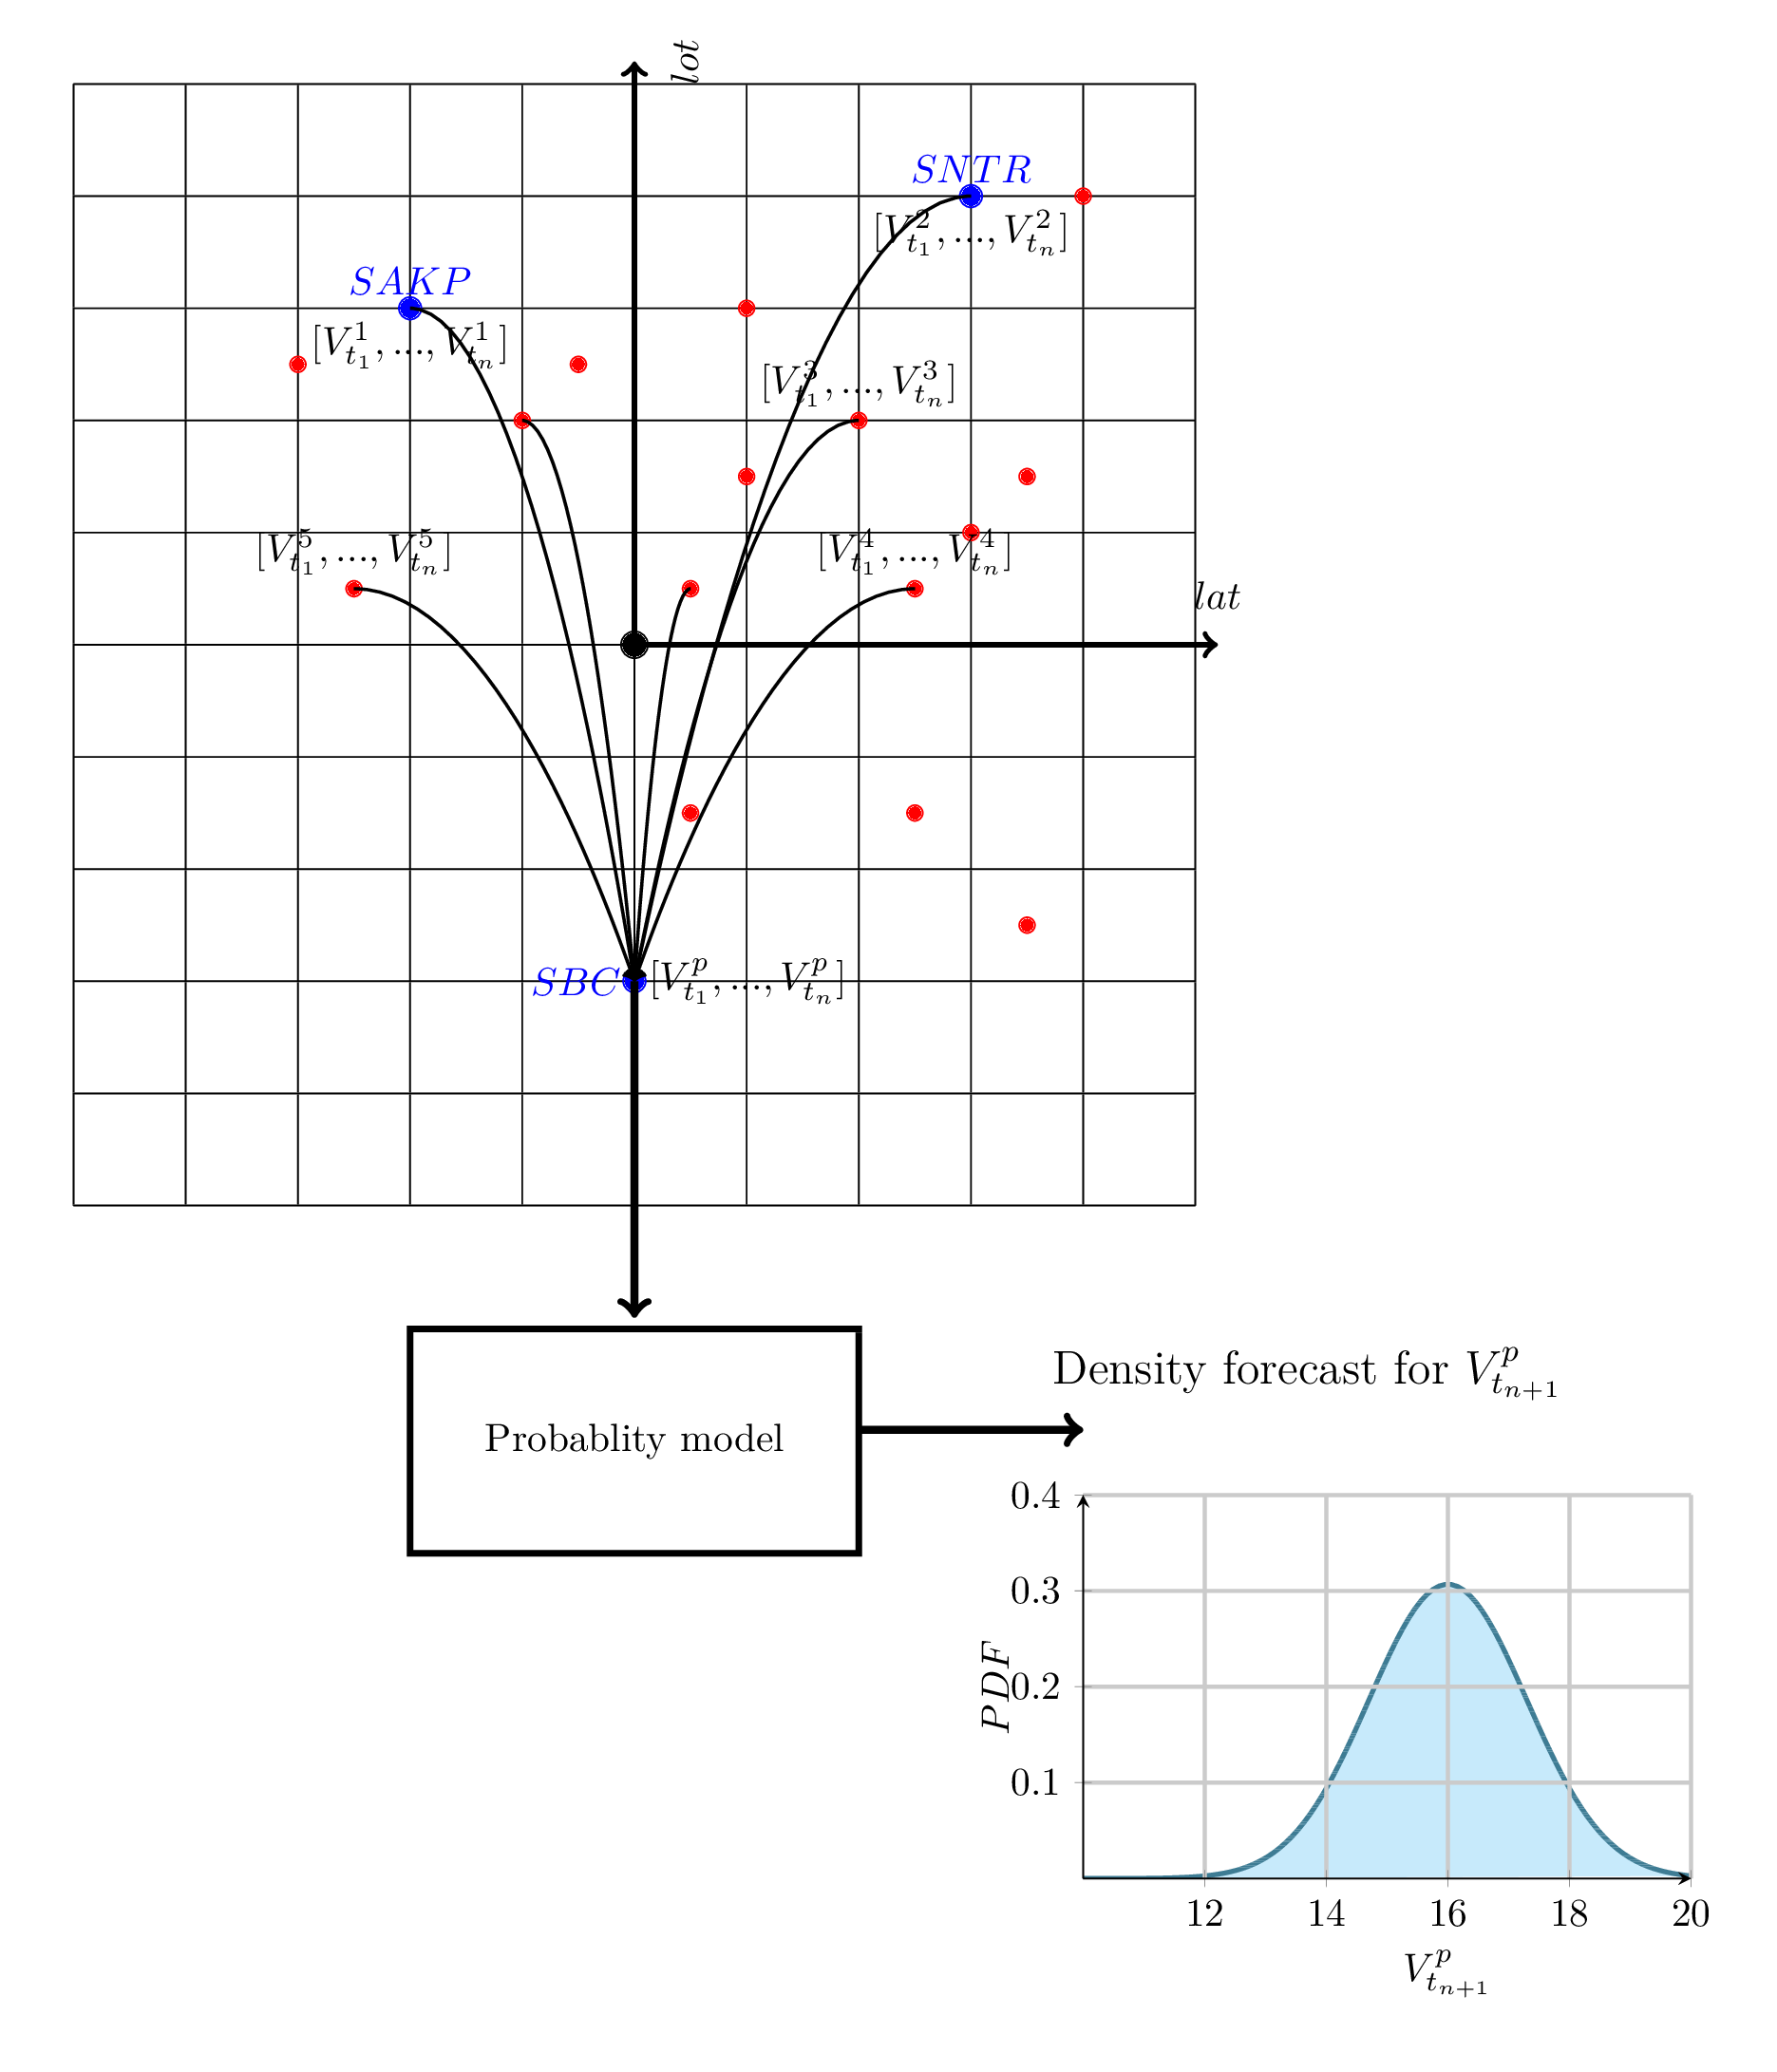
\includegraphics[height=1\textwidth, width=1\textwidth]{figures/general_system.png}
    \caption[General system]{General view of the system we aim to build. The red dots represent unreliable DYI sensors. Data from all the sensors is used in order to make prediction for one (SBC) of the LUBW-Stations (shown in blue). The prediction made is for some future moment \(t+1\) and it is made on the basis of the past - the values of all moments till \(t+1\) from all the stations. The prediction is generated in form of a probability distribution generated by the probabilistic regression model. }
  \end{figure}
\end{center}

\subsection{Probabilistic regression}
\label{sec:prob-regression}

Regression models make real valued predictions given an input data point and based on training data. Each time a prediction is made, one would desire to have a certain measurement for the uncertainty of the prediction. If this is the case and the prediction is given in a form of some distribution we say that the forecast is probabilistic. This quantification of the uncertainty allows for optimal decision making. Models that produce such probabilistic forecasts have gained recent popularity in areas such as meteorology, seismology and economics (see \refsec{sec:related-work} for concrete examples).

Probability forecasts are not uncommon for classification models. Through the use of soft-max layer (see \cite{denker1990}) neural networks can assign each class they recognize a certain probability. This thesis is centered however around probabilistic regression models. \emph{Probabilistic regression models} produce a probability distribution as their prediction rather than a point estimate. One can then draw samples form this distribution, make statements about the drawn samples and reason about the nature of the possible values that could be predicted. Illustration of this is given in \reffig{fig:pred-dist-draws}. Another way of thinking about probability forecasts is that they define a certain region where the actual value can be. The region however is a probability distribution. The model tells us then what the probability of each realising value given the input by evaluation is. We say that the model describes the conditional probability of the output given the input (more details in \refsec{sec:prob-modeling}). \reffig{fig:prob-regression} illustrates these considerations about probabilistic regression models. 

Predicting distributions rather than point estimates also plays a role in the evaluation of the predictive capabilities of a given model. Because the prediction is distribution, its evaluation requires different measures of predictive performance. \reffig{fig:point-vs-dist} illustrates the apparent difference between point estimate and distribution prediction and how can one can reason much more if a distribution for the prediction is present. In our evaluation of the models we employ proper scoring rules (see \cite{rafteryg2007}). They evaluate the error between a predicted probability distribution and a realized observation. We give more details on the proper scoring rules in \refsec{sec:proper-scoring-rules}.

\begin{center}
  \begin{figure}[htbp]
    \label{fig:pred-dist-draws}
    \centering
    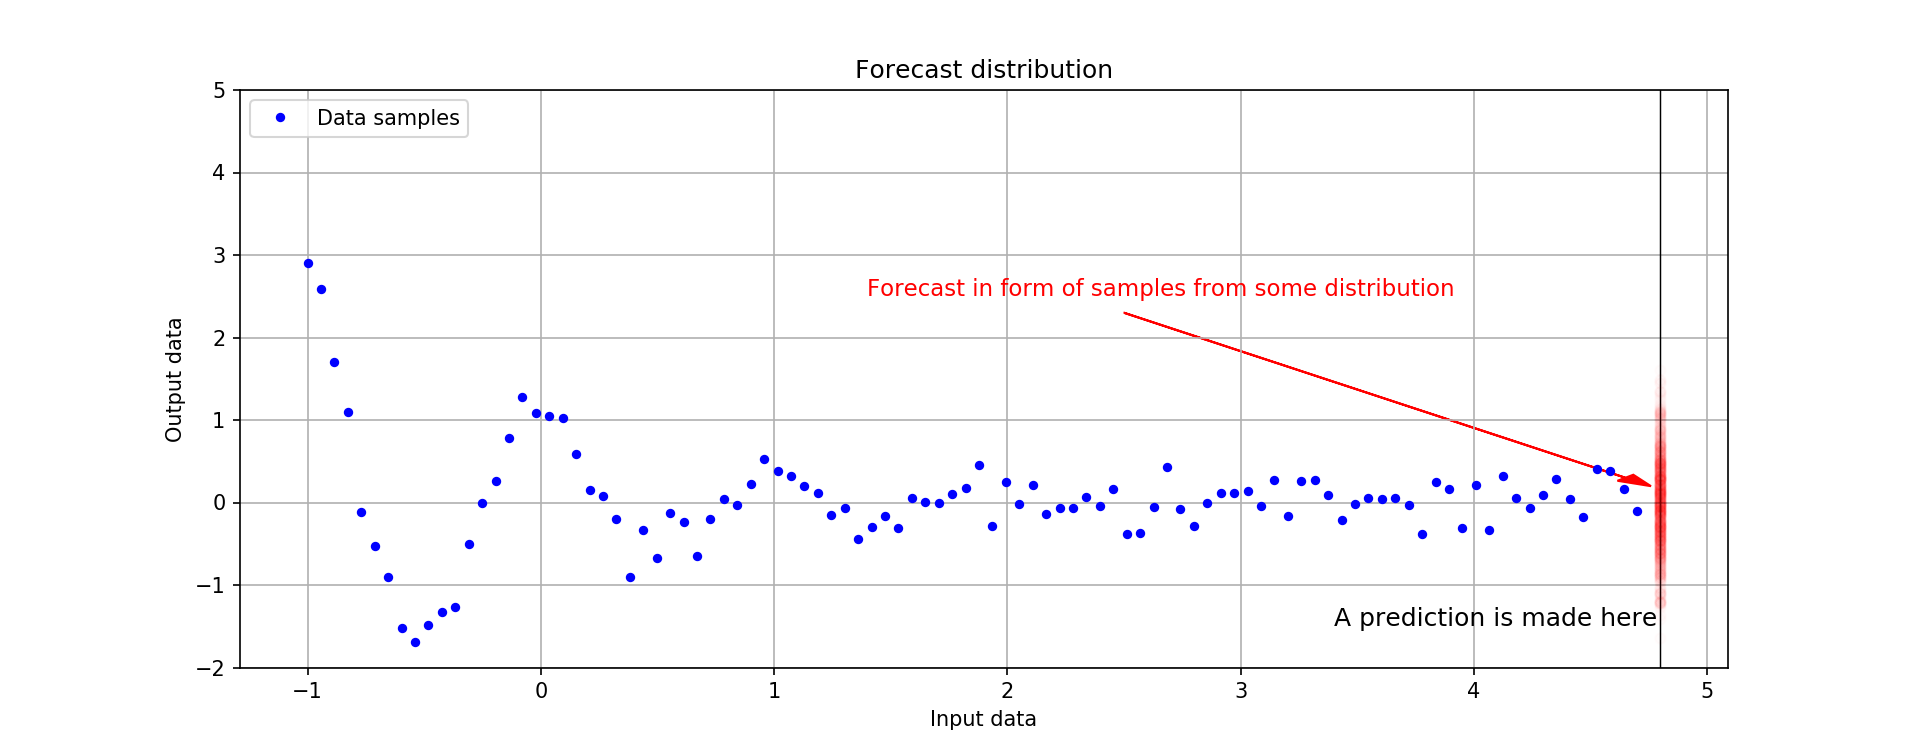
\includegraphics[height=0.5\textwidth, width=1.0\textwidth]{figures/forecast.png}
    \caption[Forecast sample draws]{Illustration of what samples from forecast could look like. The blue dots are observations. On their basis a prediction is made. The red dots are drawn samples from the predicted distribution. We can see that those are concentrated near the most probable value of the observation at this place.}
  \end{figure}
\end{center}

\begin{center}
  \begin{figure}[htbp]
    \label{fig:point-vs-dist}
    \centering
    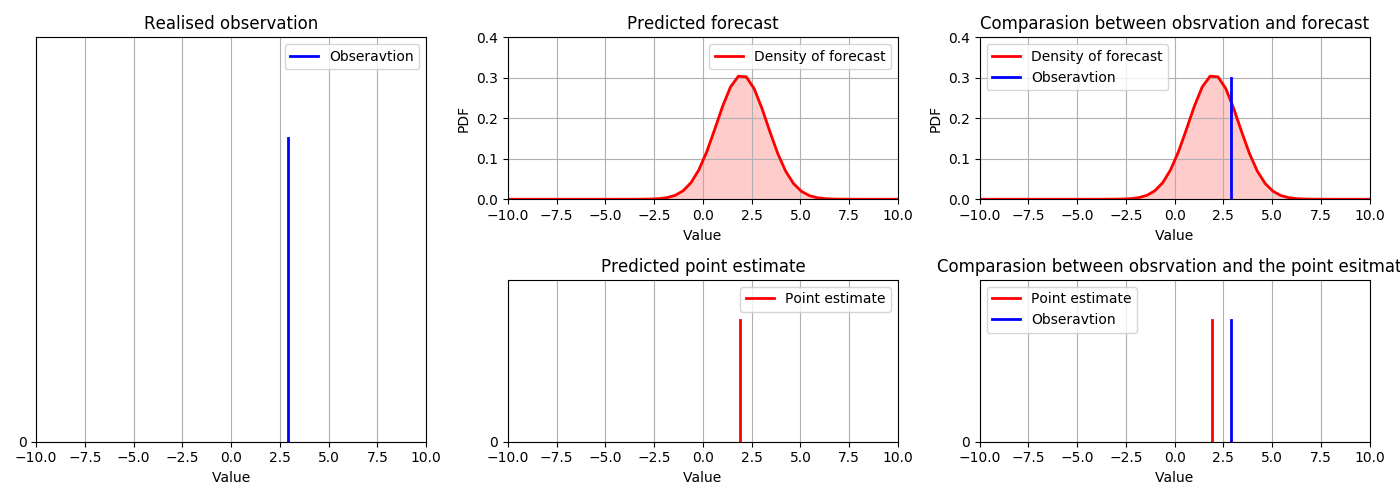
\includegraphics[height=0.5\textwidth, width=1.0\textwidth]{figures/distribution_point.png}
    \caption[Point estimate and distribution forecast]{The left most graph shows actual observation that is to be predicted. In the middle there are two prediction made by two different models - a probabilistic forecast (on the top) and point estimate(on the bottom). With the right graphs one can clearly see how there is not a whole lot to compare between the point estimate and the observation other than the distance between the two. With the probability forecast however we can evaluate where and how exactly fits the observation in the predicted distribution.}
  \end{figure}
\end{center}

\begin{center}
  \begin{figure}[htbp]
    \label{fig:prob-regression}
    \centering
    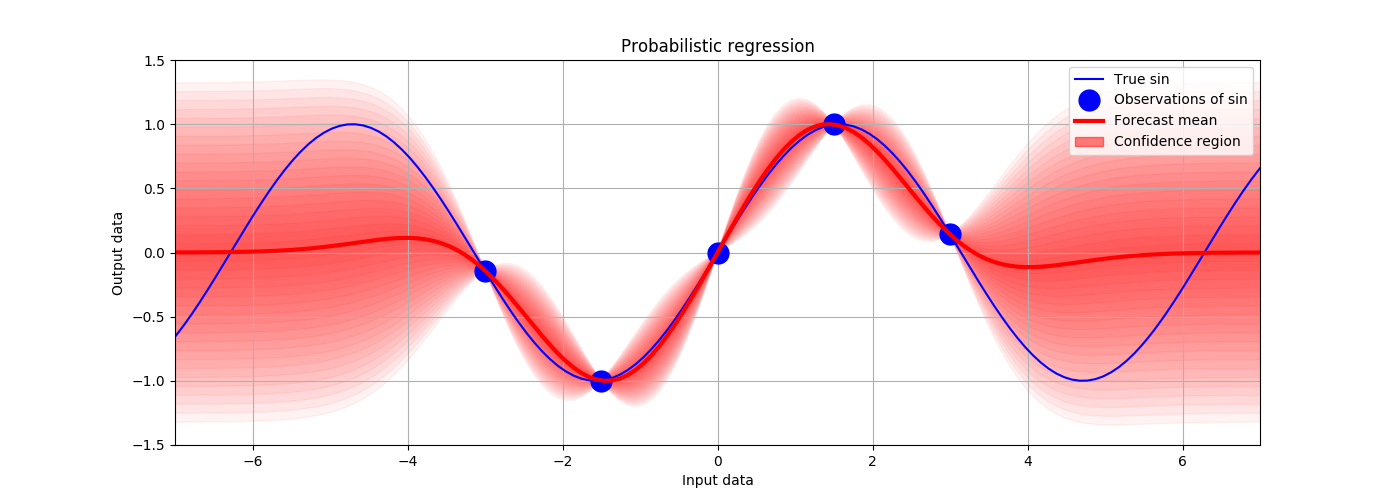
\includegraphics[height=0.5\textwidth, width=1\textwidth]{figures/probabilistic_regression.png}
    \caption[Probabilistic regression example model]{A probabilistic regression model (in red) that tries to model the \(\sin\)-function (in blue). The big blue circles are the observations of the function that the models becomes as training set. On the basis of those observations we construct a probabilistic model that can evaluate the whole input space. The model knows about the given observations of the modeled function so it predicts their values with high certainty. The places where there is no observed data however, the model cannot make precise prediction and the distributions is wider. We notice however that true value of the function lies in the distribution so in sense the model predicts the function somewhat accurately. } 
  \end{figure}
\end{center}

The quality of probabilistic forecasts also have two other important characteristics:
\begin{itemize}
\item Calibration - This is measure of the compatibility between the forecast and the observation. It depends both on the observation and on the  forecast in form of probability distribution.
\item Sharpness - Concentration of the forecasts. This property is purely of the distribution.
\end{itemize}
We look at those again in detail in \refsec{sec:prob-modeling}.

The statistical framework for inferring probability distributions is \emph{Bayesian Inference}. A good theoretical and practical overview of Bayesian inference can be found in \cite{tipping2004}. In Bayesian inference Bayes theorem (see \cite{bayes63}) plays a central role in determining the probability for a hypothesis given some evidence. Bayesian inference takes into consideration our prior beliefs about the nature of some data and then combines those beliefs with the actual observed data (denoted as \emph{evidence}) and generated \emph{posterior} probability about the values of the output. We discuss Bayesian reasoning in \refsec{sec:bayesian-inference}.

\subsection{Data}
\label{sec:data}

As previously stated, the used data comes from two different types from sources.
\begin{itemize}
\item \href{https://www.lubw.baden-wuerttemberg.de/startseite}{LU-BW} (Landesanstalt für Umwelt, Messungen und Naturschutz Baden-Württemberg) - Organization whose activities include air measurements and high quality sensors deployment. LUBW has gathered data from 3 high quality sensors in Stuttgart for the year 2017. The data is to be used for research proposes only and is not publicly available.
\item \href{https://luftdaten.info/}{luftdaten.info} - a public network of sensors where everyone can provide data from sensor from certain type. There we can find air pollution data from \emph{sds011}-sensors (see \cite{sds011}  for specifications). Those are cheap DIY sensors and give no guarantees for the quality of the measured data. Measurements of wide networks of such sensors are publicly available under \cite{datalink}.
\end{itemize}
All of the sensors measure two types of air pollution data. The different naming of those values relates to the size of the measured particles. The two data types are:
\begin{itemize}
\item \emph{PM2.5} - Particular matter up to 2.5 micrometers.
\item \emph{PM10} - Particular matter up to 10 micrometers.
\end{itemize}
We found that those values are highly correlated - correlation of about 0.95 on average (see \refsec{sec:preprop-data} for details). For this reason the built models use either PM2.5 or PM10. That is, with PM2.5 data of all other sensors, we predict the PM2.5 values of a particular sensor or respectively with PM10 data we predict PM10 values.

The format of the data coming straight from the networks was not convenient for direct training of the models. The sensors from \emph{luftdaten} provide measurements for each minute over the whole year while the ones of LUBW integrate their measurements over thirty minutes. Because of this inconsistency we had to ``synchronize'' the both data sources in order to produce the final data sets. We've also found numerous problems with the data from \emph{luftdaten}. Some of them are:
\begin{itemize}
\item Not all sensors are located around Stuttgart.
\item Some of the sensors have a lot of missing days without measurements.
\item Some of the sensors have missing measurement in random minutes of the day.
\end{itemize}
The raw data was extensively prepossessed with different techniques. In \refsec{sec:impl} we describe all of the steps taken to achieve that.
%We wanted to clean the noisiness out of the data in order to make it as simple to models as possible while still retaining the relevant information.
\subsection{Models}
\label{sec:models}

The models of interested that we are going to look at are \emph{Bayesian Neural Networks} (\emph{BNNs}, see \refsec{sec:bnn}) and \emph{Mixture Density networks} (\emph{MDNs}, see \refsec{sec:mdn}). Here we give brief overview of the both models and we discuss them in detail in the respective sections.

BNNs are relatively new type of model proposed in the 1990s and studied in depth in \cite{mackay1992}, \cite{neal1996}. \cite{gal2016} provides general survey and study on  of uncertainty quantification in deep learning. More recently BNNs have seen a surge in popularity as they combine Neural Networks with Probabilistic Models.The inferred distributions over their wights allows them to offer a probability distributions for their estimates. This makes BNNs attractive to the machine learning community as those properties give them robustness to over-fitting and ability to learn from small datasets. BNNs place prior distribution on their weights. The posterior distributions are estimated either by variational inference (\cite{blundell2015},\cite{paisley2012}) or by sampling techniques (\cite{vehtari2000}). In our work we use variational inference with \emph{Kullback-Leibler divergence} and give details about the method in \refsec{sec:var-inference}.

With MDNs we hope to construct a model similar to mixture of Gaussian  experts similar to \cite{rasmussen2002}. The mixture of Gaussian experts is a combination of several Gaussian Process regression models and a gating network. Given an example data point the gating network assigns certain probabilities for each of the Gaussian process models. On their turn they generate several probability distributions which are weighted with the probabilities from the gating networks. The end result again is a probability distributions given by the sum of the individual ones. MDNs model this by creating a single network that not only outputs weights for the individual mixture components but also their parameters. MDNs are very similar to standard Neural Networks with the only difference being that final layer is mapped to a mixture of distributions. In our case the mixture model is a weighted sum of Gaussian process regressors. MDNs produce especially good results when the input data is such that a single input can correspond to multiple output values. In those cases, the predicted distribution models the corresponding output values by giving some probability on each of them. We investigate what results one can get when this approach is used for simpler data. As MDNs are almost standard neural networks, they are trained with the standard \emph{backpropagation} method, described for example in \cite{bertels2001}.

In order to have a baseline with which we can compare the build models we also construct simple empirical model. The empirical modeling technique for prediction of values based on empirical observations. In this cases there is no consideration of the input of the data but rather a simple looking at the past values of the output value. The past values of the predicted measurement are treated as samples from a random variable. We describe how we infer a probability distribution for a prediction in \refsec{sec:impl-model}. Similar empirical models are commonly used for simple predictions of meteorological data (see \cite{krueger2011} and \cite{eden2015}). 

\section{Related work}
\label{sec:related-work}

Heterogeneous sensor networks are not uncommon. \cite{wu2007} looks at the deployment and the topology control specifically of Heterogeneous Wireless Sensor Networks. \cite{katiyar2010} surveys a variety of clustering algorithms aimed at increasing the  network's scalability by recognizing the sensors with similar energy requirements. \cite{uplap2014} investigates the kinds of security threats that arise with the use of heterogeneous sensor networks. In the context of machine learning \cite{liu2017} tries to use deep learning techniques and adapt them to the settings of heterogeneous sensor data.

A lot of attention has been brought to probabilistic forecasting(\cite{gneiting2014}). When it comes to history, \cite{stigler1975} describes the transition from point estimates to distribution prediction. Nowadays the technique is widely used in variety of cases as it is further developed (\cite{ehm2012}). Common areas  where probabilistic forecasts are employed are whether and climate  prediction ( \cite{collins2007}). The uses are however not limited only to that. \cite{krzysztofowic2001} looks how probabilistic models could be used for flood risk assessment, \cite{timmermann2001} deals with economic and financial risk management, \cite{pinson2013} tries to make predictions about the availability of renewable energy resources. Distribution forecasting could be even used to make statements about the outcome of elections (\cite{montgomery2012}).

The other focus of our work are BNNs. As models that tie Bayesian reasoning and neural networks (\cite{schmidhuber2015} presents good overview of NN and deep learning) together, they have also gained popularity. \cite{vehtari2001} first gives brief overview of the Bayesian approach to neural networks and then surveys different use cases assessing the performance. Fields like astrophysics \cite{bai2016} and particle physics \cite{bhat2015} also profit from the predictive capabilities of BNNs. As medicine is one of the fields that gets much of the attention of the machine learning research, \cite{kwon2017} applies BNNs in order to quantify the uncertainties and apply them in ischemic stroke lesion segmentation. BNNs are also continuing to be developed. \cite{fortunato2017} explores the Bayesian approach in Recurrent Neutral Networks developing \emph{Bayesian Recurrent Neural Networks}.

MDNs have also found popularity as one another alternative to combine neural networks with distribution forecast models. \cite{schittenkopf1998} treat MDNs as a general framework for identifying stochastic processes and apply them in modeling stock exchange index data. \cite{zen2014} bring MDNs to use in order to improve deep neural networks for acoustic modeling. MDNs have their own variant of recurrent models as described in \cite{miazhynskaia2003}. We like to note that  MDNs have similar structure to other models such as \emph{Adaptive mixture of local experts} (\cite{jacobs1991}) and \emph{Infinite Mixtures of Gaussian Process Experts} (\cite{rasmussen2002}) but are different in their way of modeling data (as explained in \refsec{sec:mdn}).

The use of proper scoring rules is not uncommon in  probability forecast setting. \cite{jordan2017} discusses the \textbf{scoringRules} package for R (programming language) and its usage details by presenting case studies where proper scoring rules find application. \cite{clements2004} uses probability integral transform (see \refsec{sec:disp-sharp}) in order to evaluate the UK Monetary Policy Committee's inflation density forecasts.
% \cite{friederichs2012} deals specifically with verifying predicted probability distributions under the use of proper scoring rules.

\section{Probabilistic Modeling}
\label{sec:prob-modeling}

\subsection{Bayesian regression modeling}
\label{sec:bayesian-inference}
In probabilistic modeling we try to estimate parameters of given model by first defining some prior on them. The prior distribution describes, how likely values of the parameter are without considering any observed data. Then a \emph{conditional likelihood} for the output based on the parameters and the input data is defined. This posterior probability distribution describes the probability of observing certain data given the parameters of the model and under the assumption that the models has generated the data . The two distributions are then combined in order to produce the final posterior on the parameters of the model. A very detailed look at Bayesian models in the context of Gaussian processes can be found in \cite{rasmussen2005}. We can summarize:
\begin{itemize}
\item \textbf{Prior} - uncertainty in form of probability distribution \emph{before} observing the data.
\item \textbf{Posterior} - uncertainty probability distribution \emph{after} observing the data.
\end{itemize}

Now we formally write down everything following \cite{gal2016}. Let
\begin{equation}
  X = \{x_1,..., x_N\}, \forall i : x_i\in\mathbb{R}^M
\end{equation}
be the set of input data. The corresponding output is  given by the set \(Y = \{y_1,..., y_N\}\). The dataset could also be seen as tuples of feature vector \(x_i\) and an output value \(y_i\). We can then write the dataset as \(\{ (x_i,y_i)\}_{i=1}^N \). As we deal with regression models we assume that  \(\forall i : y_{\text{i}}\in \mathbb{R}\) and there exists some function \(f:X \rightarrow\mathbb{R}\) with \(f_{true}(x_i)=y_i, \forall i \in\{1,..., n\}\). We want to find a model with appropriate parameters that is likely to have generated the data. In fact, through choice of parameters, we want the data to be as probable as possible according to the defined model. We model the mapping function between \(X\) and \(Y\) through a separate function \(f_m(x; \omega)\) parameterized by \(\omega\). We want to find a ``good'' set of parameters \(\omega\) such that the function \(f(x;\omega)\) is \emph{likely} to have generated the output data. We define our prior believes about the parameters through the distribution  \(p(\omega )\). The generalized likelihood distribution is then  \(p(y|x, \omega)\). That is, how likely is output \(y\) given  model parameters \(\omega\) and concrete input \(x\). Our assumption here is that the defined model generates the data. The output of a regression model is typically set to be a  Gaussian likelihood: \(p(y|x,\omega)=\mathcal{N}(y; f_m(x;\omega), \tau^{-1}I)\) where \(\tau\) is the  model precision. This can be interpreted as adding small amount of noise to the output as modeled in \cite{gal2016}.

We can now  write out the posterior by using the Bayes' theorem:
\begin{equation}
p(\omega|X,Y) = \frac{p(Y|X, \omega)p(\omega)}{p(Y|X)}
\end{equation}
This distribution models the most probable function parameters given the observed data. If we choose the parameters from this distribution the observed data will be most likely. For prediction of new data point \(x^*\) we use  \(p(y^{\text{*}}|x^{\text{*}},X,Y) = \int p(Y|X, \omega)p(\omega)d \omega\). This integration is called \emph{inference}(\cite{gal2016})). The quantity
\begin{equation}
 p(Y|X) = \int (Y|X, \omega)p( \omega )d \omega
\end{equation}
is called marginal likelihood or sometimes ``model evidence''. The first name comes from the fact that we are marginalizing the likelihood over \(\omega\). This factor is independent of the parameters so no matter how we choose them, it does not change. Marginalization plays central part in Bayesian modeling and in the prefect case we would want to marginalize over all possible parameter values  \(\omega\) with respective weight \(p(\omega)\). In complex models this is not possible and we resort to approximations.

``Learning'' in this Bayesian setting boils down to finding the posterior distribution \(p(\omega |X, Y)\) over the parameters. In the general case this cannot be done analytically (a closed formula cannot be given) and thus one must attempt to approximate the distribution.

Inference provides us with the full probability distribution over the parameters and for that reason we are not dealing with point estimates of the parameters. By extension we could also provide some distribution when we evaluate the model on unseen data. In order to ``generate'' a sample from the resulting distribution for some unseen input data point \(x^*\) we first need to sample \(\omega_s\) from the parameter distribution and then evaluate the model \(f_e\) at point \(x^*\) parameterized by the drawn sample  \(f_e(x^*; \omega_s)\).

The models that we look next are nothing more than concrete choices for \(f_e(x;\omega)\)
\subsection{Bayesian Neural Networks}
\label{sec:bnn}
\subsubsection{Neural networks}\label{sec:nn}
\noindent\emph{First we give brief overview of conventional neural networks.}

Neural networks (or artificial neural networks) are computing systems that model certain function structure. Neural networks consist of artificial neurons that have a certain number of inputs. They first compute weighted linear sum of their inputs and then apply non-linearity (in form of \(\tanh\), logistic or other type of \emph{sigmoid} function). Several stacked neurons are considered network layers. Several consecutive layers where the output of one layer is the input of the next are considered a \emph{neural network}.

Formally the neural network is nothing more than a parameterized function with specific structure that allows it to estimate almost every possible function when given the right parameters. Let \(W_i \in \mathbb{R}^{A_i \times B_i }\) and \(b_i\mathbb{R}^{B_i}\) be weight matrices and biases respectively and let \(o_i\mathbb{R}^{B_i}\) denote the output of the \(i^\text{th}\) layer of the network. For an input \(x \mathbb{R}^{A_1}\) we then have:
\begin{align}
  o_{1} &= \tanh((W_{1}x) + b_{1}) \\
  o_{2} &= \tanh((W_{2}o_1) + b_{2}) \\
        &\vdots
\end{align}
In general, for a network with \(m\) layers where the \(m^{\text{th}}\) layer is the output layer, the outputs of the individual layers can be given as:
\begin{align}
  \label{eq:nn-ouput}
  o_{i+1}  &= \tanh((W_{i+1}o_i) + b_{i+1}) \\
  o_m     &= (W_{m}o_{m-1}) + b_{m}
\end{align}
where \(o_m \) is the final output of the network. The forward evaluation of the network is just a cascade of applications of liner functions in form of matrix multiplication and additions of bias followed up by application of some non-linear function. For sake of simplicity let us collapse the notation of the output  of the network to a single function of the input \(x\) and the collection of parameters (weight matrices and bias-terms) \(\Omega\). With the evaluation of the netowork can be given with
\begin{equation}
    o_m = f_{net}(x; \Omega)
\end{equation}
In order to be useful we have to ``teach'' the neural network our desired mapping. As in previous section we have a set of input data \(X = \{x_1,..., x_N\}, \forall i : x_i\in\mathbb{R}^M\) and the corresponding output for each \(x_i\) is contained in the set for the output data \(Y = \{y_1,...,y_N\}, \forall i : y_i\in\mathbb{R}\). Ideally we would want the following to hold for the neural network
\begin{equation}
  f_{net}(x_i;\Omega) = y_i
\end{equation}
In other words, the network have \emph{learned} the exact mapping between \(X\) and \(Y\) and can predict the output value based on the input one. This is done by choosing appropriate parameter set \(\Omega\). In general, finding parameters realising the exact mapping will not be possible but we want to at least approximate this case. This leads us naturally to a definition of measurement of just how wrong the network is. We call this quantity \emph{error function} (also called \emph{loss function}). The error function is a function of the parameter space and it is closer to zero if the given parameters of the network are better in modeling the output. There are lot of possible choices for loss function but the most common is the \emph{squared error difference}:
\begin{equation}
 E(\omega) =  \sum_{i=0}^N (f_{net}(x_i;\omega) - y_i)^2
\end{equation}
Here \(\omega\) is some choice for the parameters for the networks, namely \(m\) weight matrices and \(m\) bias terms for network with \(m\) layers. Minimizing this \emph{error function} is what we call \emph{learning} the data or \emph{training} the network. The actual method trough which learning occurs is backpropagation. This involves calculating the derivatives of the loss function with the respect to each parameters of the network \(\frac{\partial E}{\partial W_i }\). The corresponding parameters are then updated through some gradient descent (see \cite{ruder2016} for overview) technique. Some state of the art optimization methods are \emph{LM-BFGS} (Limited Memory Broyden–Fletcher–Goldfarb–Shanno algorithm, \cite{byrd1995}), Adam optimization algorithm (see \cite{kingma2014}) and \emph{SGD} (Stochastic gradient descent,\cite{robbins1951}). To note is that the last motioned method - the SGD - does not calculate the gradient of the loss function using all of the training examples rather it uses only a small subset of the training set.

We would like to note that neural networks are often considered as universal function approximator. This means that given enough complexity of their structure, they can model arbitrary non-linear functions (see \cite{hornik1989}).
\subsubsection{Neural networks in Bayesian settings}
\label{sec:nn-in-bayesian}
\noindent\emph{We now focus on what Bayesian neural networks are}.

BNNs place a prior distribution over the parameters of a neural network. As described in previous section, once we have distributions on the parameters of a model, we have effectively defined a distribution of functions\footnote{Each time when we draw a sample from the parameter space, we have defined a ``new'' function that models the given data. In this sense, we have sampled a new function from some distribution.}. Usually, for given weight matrix \(W_i\) and bias term \(b_i\) in layer \(i\) of the network, BNNs place standard Gaussian prior distributions over the matrices, \(p(W_i)=\mathcal{N}(0,I)\) and a point estimate for the \(b_{\text{i}}\) is assumed. In this work, however, the standard prior is also placed on the bias vectors so we define the distributions \(p(b_i)=\mathcal{N}(0,I)\).

As at their core BNNs are neural networks, we will use the notations from above. The output of the network for a given input \(x\) and parameters \(\Omega\) is
\begin{equation}
   f_{net}(x;\Omega)
\end{equation}
At this moment we have defined what the basic structure of our considered model is (neural network) and know what the priors of the parameters over the model are. As in the previous section we now define a likelihood for each data point. We consider set of data \(\{(x_i, y_i), i\in\{1,...,n\} \}\) where each data point has some features \(x_i\in\mathbb{R}^M\) of dimension \(M\) and real valued output \(y_i\in\mathcal{R}\). We define the likelihood for the BNNs as:
\begin{equation}
  p(y_i|\Omega, x_i, \sigma^2) = \mathcal{N}(y_i |f_{net}(x_i;\Omega), \sigma^2)
\end{equation}
where \(\sigma^{\text{2}}\) is again some known small variance that can be considered as ``noise'' of the output (\cite{gal2016}).

With this overview we can make several general statements about BNN. A BNN is a probability model that utilizes a neural network as universal function approximator. The distributions on the network's parameter allow it to generate a distributional output rather than a point estimate. This the exact same Bayesian setting as described in \refsec{sec:bayesian-inference}. 

The final piece of having some useful model is to have notion what ``learning'' means in the case of BNN. As this is Bayesian probability model we have to find the posterior distribution over the parameters based on the example data:
\begin{equation}
  p(\omega|Y,X)=\frac{p(Y|X,\omega)p(\omega)}{p(Y|X)}
\end{equation}
This distribution describes the most likely parameters given the example data. Direct computation of the posterior is not possible for networks of any practical sizes. The problems come from the term in the denominator as it involves integrating over the whole parameter space:
\begin{equation}
  p(Y|X) = \int_{\Omega} p(Y|\omega , X)p(\omega|X)d \omega
\end{equation}
In the next section we describe a technique that aims to estimate the posterior distribution without actually having to approximate the above integral. Once we have the posterior distribution (or a sufficient estimate of it) we could use it to produce the predicted distribution for unseen data samples. This is done through \emph{inference} as described in \refsec{sec:bayesian-inference}.

\subsubsection{Variational inference and Kullback-Leibler divergence}\label{sec:var-inference}
As previously stated, it is impractical to compute the full posterior. In fact the true posterior is intractable and cannot be evaluated analytically. We therefore rely on an estimation technique that transforms the Bayesian inference into a optimization problem - \emph{variational inference} (first proposed in \cite{jordan1999}, see an overview in \cite{blei2016}, a detailed look in \cite{fox2012}). We define a \emph{variational} distribution \(q_{\theta}(\omega)\), parameterized by \(\theta \). We assume that this distribution is easy to evaluate. Furthermore we would really like this distribution to be able to approximate other distributions based on the choice of parameters \(\theta\). If those assumptions are met, we then try to choose such parameters for \(q_{\theta}(\omega)\) that it maximally resembles the posterior \(p(\omega|Y,X)\). For that we also need some measure between two distributions that gives us how ``similar'' they are. This is slightly analogous to the choice of loss function that is to be minimized. In this case we use the \emph{Kullback–Leibler} (KL) divergence proposed by \cite{kullback1951}. KL is defined as


\begin{equation}
  KL(q_{\theta}(\omega), p(\omega | X, Y)) = \int q_{\theta}(\omega) \log \frac{q_{\theta}(\omega)}{p(\omega | X, Y)}d\omega 
\end{equation}
KL is a measure of how one probability distributions differs from another. A Kullback–Leibler divergence of \(0\) implies the two distributions are identical and it does not have a maximum as it is unbounded. We aim to minimize this function with respect to \(\theta\). Our problem then becomes:
\begin{align}
  \theta^* &= \underset{\theta}{\arg\min} \,  KL(q_{\theta}(\omega), p(\omega | X, Y))\\
           &= \underset{\theta}{\arg\min}\, \int q_{\theta}(\omega) \log \frac{q_{\theta}(\omega)}{p(\omega | X, Y)}d\omega \\
           & = \underset{\theta}{\arg\min}\,  KL(q_{\theta}(\omega), p(\omega)) - \mathbb{E}_{q_{\theta}(\omega)}[\log\, p(Y|w)]
\end{align}
The last cost function is known the \emph{variational free energy} (\cite{neal1998},\cite{blundell2015}) or the \emph{expected lower bound} (\cite{fox2012}, \cite{saul1996}). Thus the function that we want to optimize is
\begin{equation}
  \mathcal{L}(\theta, Y) = KL(q_{\theta}(\omega)||p(\theta)) + \mathbb{E}_{q_{\theta}(\omega)}[\log(p(Y|\omega))]
\end{equation}
This loss function is a sum of a data-dependent part  and a prior-dependent part. The function embodies a trade-off between satisfying the complexity of the data - \(X \text{ and } Y \) - and satisfying the simplicity of the prior \(p(\omega)\)(\cite{blundell2015}).


Gradient calculation of this function is not a trivial task. As we do use standard Gaussian priors on the parameter \(\omega\), the first term in the function (the KL divergence) is traceable and analytically solvable (\cite{paisley2012} ). For the actual implementation of the optimization we use \cite{tf} (more details in \refsec{sec:impl-model}). The other term however, is not that well behaved. Several methods have been proposed to optimize the function with backpropagation techniques. The concrete implementation that we (\cite{edward}) use, utilizes either \emph{Stochastic Gradient Vitiation Bayes} (\emph{SGVB}) as described in \cite{kingma2013} or the method described in \cite{paisley2012}. 
 

To give brief overview of SGVB - for the approximate posterior \(q_{\theta}(\omega)\) we reparameterize the random variable \(z \sim q_{\theta}(\omega)\) by the use of some differential transformation \(g_{\omega}(\epsilon , x)\) and a noise variable \(\epsilon\).
\begin{equation}
  z =  g_{\omega}(\epsilon , x), \quad \epsilon \sim p(\epsilon)
\end{equation}
With those definitions we can now estimate the exception of some function \(f(x)\) with respect to \(q_{\theta}(\omega)\):
\begin{equation}
  \mathbb{E}_{q_{\theta}(\omega)}[f(x)] = \mathbb[f(g_{\omega}(\epsilon , x))] \simeq \frac{1}{L}\sum_{l=1}^L f(g_{\omega}(\epsilon^{(l)} , x))
\end{equation}
We could apply this technique to our cost function and we get a tractable  differentiable  estimate of it
\begin{equation}
  \mathcal{L}(\theta, Y) \simeq \mathcal{L}(\theta,Y)^E = KL(q_{\theta}(\omega)||p_{\theta}(z))  + \frac{1}{L}\sum_{l=1}^L(\log(p_{\theta}(x|\omega)))
\end{equation}
Now that we have a function for which the gradients could be given analytically, we could optimize it with respect to the parameter \(\theta\). This is done typically through Stochastic Gradient Descent (see \refsec{sec:nn}). In this case we do not calculate the loss on the whole dataset but rather on s sub-sample of it. Lets say we take \(M\) datapoints from dataset with \(N\) datapoints. Then essentially we are making the estimate:
\begin{equation}
  \mathcal{L}(\theta, Y) \simeq \mathcal{L}(\theta, Y^M)^E_M = \frac{N}{M}  \sum_{i=1}^{M}\mathcal{L}(\theta, y_i)^E
\end{equation}
It is known that SGD leads to faster convergence with less computations (\cite{robbins1951}). It is also proven and observed (\cite{shapiro1996}) that SGD converges to the result of regular gradient descent. For those reasons, the usage of SGD is almost always advisable.

There is also a somewhat simpler approach of estimating the gradient of the loss function described in \cite{paisley2012}. Under some regularity conditions, a gradient of the form \(\nabla_{\theta}\mathbb{E}_qf \) where \(f \) is some untraceable function, \(q\) is some distribution and we take the gradient with respect to \(\theta\))  could be rewritten as:
\begin{align}
  \nabla_{\theta}\mathbb{E}_qf(\theta) &= \nabla_{\theta}\int_{\theta} f(\theta)q(\theta)d\theta \\
                                       &= \int_{\theta} f(\theta) \nabla_{\theta}q(\theta)d\theta \\
                                       &= \int_{\theta} f(\theta)q(\theta) \nabla_{\theta}\ln(q(\theta)) d\theta
\end{align}
The last integral can be then estimated through Monte Carlo integration (\cite{hammersley1964}). This approach could be used to replace the \(\mathbb{E}_{q_{\theta}(\omega)}[\log(p(Y|\omega))]\) in the cost function. We can then again apply stochastic gradient descent in order to spare some computations and  accelerate convergence. For more detail on the method see \cite{paisley2012}.

Other techniques for posterior estimation rely on sampling from the posterior. This can be done for example by \emph{Gibbs sampling} (\cite{geman1984}), \emph{Metropolis-Hastings} (\cite{metropolis1953}, \cite{hastings1970}) or \emph{Hybrid Monte Carlo} (\cite{duane1987}). These are all so called \emph{Markov Chain Monte Carlo} (\emph{MCMC}) methods and are not uncommon techniques. We however don't consider them here.

\subsection{Mixture Density Networks}
\label{sec:mdn}

\emph{In this section we describe an alternative approach in generating a probability model for given data set.} The first thing to consider in the  mixture density networks approach is the way we model each data point. We try to describe each data point \((x,y)\in X\times Y\) with a feature vector \(x\in\mathbb{R}^R\) and a value \(y\in\mathbb{R}\) directly through some mixture model.
 
\begin{equation}
p(y|x)=\sum_{m=1}^M \alpha_m(x)\phi_m(y|x)
\end{equation}
where \(M\) is the number of mixture components and \(\phi_m(y|x)\) is the conditional density of the \(m^{th}\) kernel. The parameters (or weights) \(\alpha_m(x)\) are called \emph{mixing coefficients} (\cite{bishop1994}). To note is that everything in the model depends on the concrete input data \(x\). In this sense the parameters for the mixture change for every data point. We choose mixture of Gaussians as with appropriate weights it can model any arbitrary distribution. This means that theoretically MDNs with Gaussian mixture can be universal distribution estimators \footnote{Similar to regular neural networks which are universal real valued function estimators}. Thus all of the density functions become:
\begin{equation}
\phi_m(y|x) = \frac{1}{2\pi^{c/2}\sigma_m(x)^c}\exp\{-\frac{\left\lVert y - \mu_m(x) \right\rVert^2}{2\sigma_m(x)^2}\}
\end{equation}
Again, the parameters of each mixture component, \(\mu_m(x)\) and \(\sigma_m^2(x)\), depend on the input data. The last equation assumes that the components of the output vector are statistically independent within each component of the distribution, and can be described by a common variance (\cite{bishop1994}). As we deal with regression in this thesis, the output vector is one dimensional and thus the assumption holds true.

With this setup, the model provides general and arbitrary conditional density function \(p(y|x)\) for the output. We treat the parameters of the mixture - the mixing coefficients \(\alpha_{\text{m}}(x)\), the means \(\mu_m(x)\) and the variances \(\sigma_m(x)\) - as continuous functions of the input \(x\). It is clear that with the proper parameter functions we can model each data point. The ``finding'' of this function is achieved through a conventional neural network which takes \(x\) as an input. This combination of mixture model and a neural network is what \emph{Mixture Density Networks} (MDNs) are. It is therefore said that MDNs are nothing more than neural network plus a mixture of Gaussians. An overview is given in \reffig{fig:mdn}

Here we again use the nice property of neural networks as universal function estimators. Before we proceed further however we must place some restrictions on the outputs of the network. Let \(z_m^{\alpha}\), \(z_m^{\mu}\) and \(z_m^{\sigma}\) be the outputs of some neural network \(f(x;\omega)\) with some parameter set \(\omega\) where \(z_m^{\alpha}\) affect the mixing coefficients \(\alpha_m\) and \(z_m^{\mu}\) and \(z_m^{\sigma}\) affect the means and variances of the mixture components respectively.

Now we give the exact relationships between the outputs and the mixture's parameters. The mixing coefficients of the mixture obviously must sum up to one as they are to be treated as probabilities:
\begin{equation}
\sum_{m=1}^M\alpha_m(x)=1
\end{equation}
We can achieve that by placing \emph{softmax} function (popularized by \cite{bridle1990}) on the respective outputs \(z_m^{\alpha} \) of the network 
\begin{equation}
 \alpha_m = \frac{e^{z_m^{\alpha}}}{\sum_{j=1}^M e^{z_j^{\alpha}}}
\end{equation}
where \(z_i^{\alpha}\) are the outputs of the networks ``responsible'' for the mixing coefficients \(\alpha_i\) 

The variances of the Gaussian distributions represent \emph{scales} and for that they must be positive. We ensure this through the use of exponential function
\begin{equation}
  \sigma_m = e^{z_m^{\sigma}}
\end{equation}
This also avoids the problem when some of the variances goes to zero. The means \(\mu_m(x)\) are to be seen as \emph{location} parameters and in order not to introduce bias in the system we model them directly with the network's corresponding outputs
\begin{equation}
  \mu_m = z_m^{\mu} 
\end{equation}
With those definitions we can summarize - for a network with \(M\) mixtures the output would be \(\{\mu_m, \sigma_m^2, \pi_m \}, m\in\{1,...,M\}\). With the outputs we can define conditional probability distribution for the data
\begin{equation}
  p(Y|X) = \sum_{m=1}^M \pi_m(X)\mathcal{N}(y|\mu_m(X), \sigma_m^2(X))
\end{equation}
Now we just have to give a loss function to be minimized. Starting from probability perspective, we want to maximize the likelihood of the the observed data \(\{(x_n, y_n)\}_1^N\), This is given by a product over the likelihoods of each data point:
\begin{equation}
  \mathcal{L} = \prod_{n=1}^N p(x_n, y_n) = \prod_{n=1}^N p(x_n)p(y_n | x_n)
\end{equation}
The term \(p(x_n)\) does not depend on the networks weights and can be spared. As for the \(p(y_n | x_n)\) - this is where the mixture model comes into play. The quantity to be maximized thus becomes
\begin{equation}
  \tilde{\mathcal{L}} =  \prod_{n=1}^N \sum_{m=1}^M \alpha_m(x_n)\mathcal{N}(y_n; \mu_m(x_n), \sigma_m^2(x_n))
\end{equation}
Maximizing \(\tilde{\mathcal{L}}\) is equivalent to minimizing
\begin{equation}
  \label{eq:log-like-sum-1}
  E = \sum_{n=1}^NE^n
\end{equation}
where \(E^n\) is the contribution of the \(n^{th}\) data point and
\begin{equation}
  \label{eq:log-like-sum-2}
  E^n = -\log(\sum_{m=1}^M \alpha_m(x_n)\mathcal{N}(y_n; \mu_m(x_n), \sigma_m^2(x_n)))
\end{equation}
This function \(E\) can be minimized with standard backpropagation technique (\cite{bertels2001}) as its derivatives are fully tractable. Exact expressions for the derivatives of \(E\) are derived and given in \cite{bishop1994} but we don't consider them here. Because the used implementation of MDNs (\cite{gpflow}) uses \emph{tensorflow} (\cite{tf}) internally, the automatic differentiation engine does the necessary work. More details in \refsec{sec:impl-model}
\begin{center}
  \begin{figure}[htbp]
    \label{fig:mdn}
    \centering
    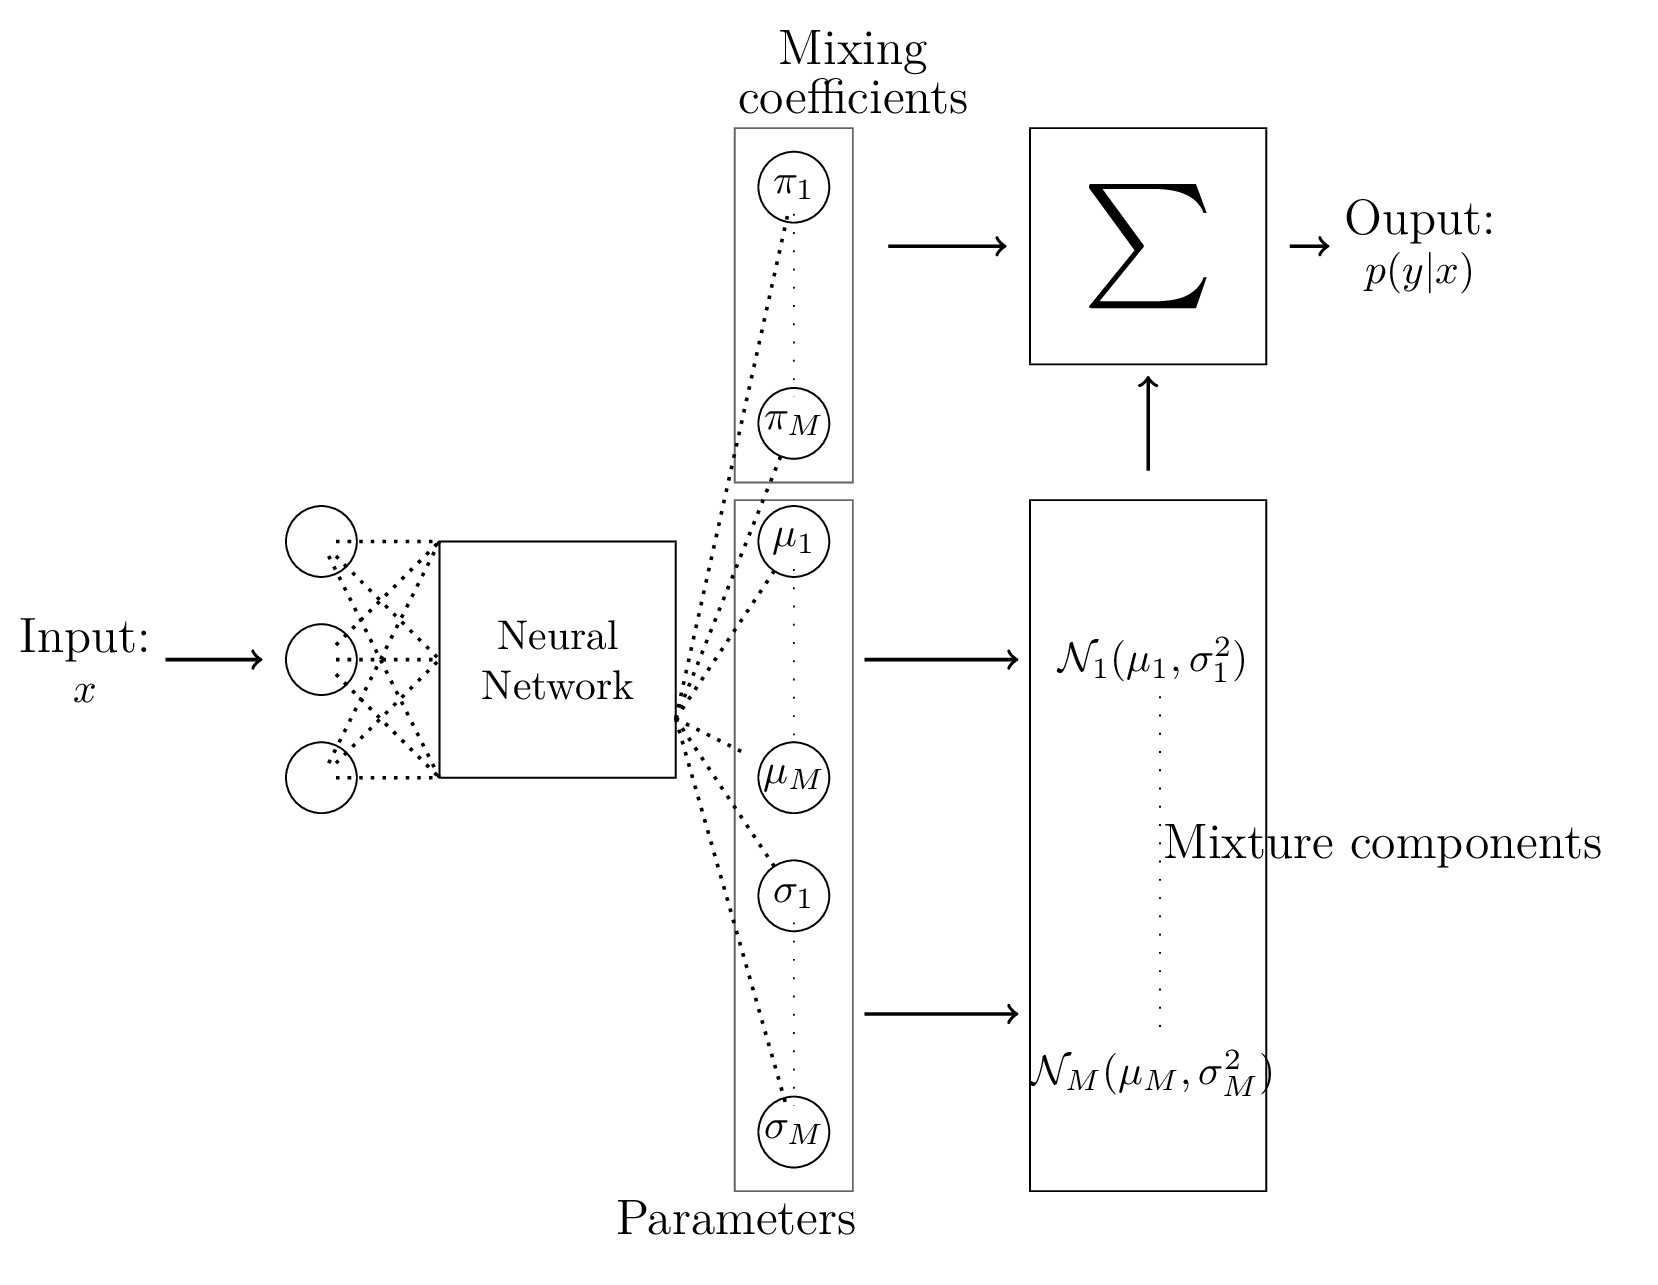
\includegraphics[height=0.6\textwidth, width=0.9\textwidth]{figures/mdn.png}
    \caption[Mixture Density Network Architecture]{Structure of a Mixture Density Network. The Input \(x\) first gets passed through a neural network. The outputs of that are treated as parameters for a mixture model. The mixture model is a weighted linear sum of different distributions - normal distributions in our case. To note is that the mixing coefficients (the weights for the sum) are also generated from the network.}
  \end{figure}
\end{center}  
\section{Model evaluation methods}\label{sec:criticism}
\noindent\emph{In this section we give formal explanation to our approach in evaluating the models we build.}
\subsection{Probabilistic Forecast}
\label{sec:prob-forecast}

\emph{First we look at more concretely how the considered stochastic models differ form classical ones.}
\subsubsection{Prediction spaces}
\label{sec:pred-space}

Classical regression models produce a point estimate \(y_i^e\) for each sample data point \(x_i\) with an actual realization \(y_i\). In this thesis however, we are interested in regression models whose output is probabilistic forecast \(F\) that can be identified with with the associated \emph{cumulative distribution function} (\emph{CDF}). This introduces the notion of prediction spaces proposed in \cite{gneiting2013}. A prediction space is a probability space tailored to the study of distributional forecasts (\cite{gneiting2014}). Formally looked we have to consider the realized observation also as distributions even thou in practice this is a single value. In the most general case, the elements of the prediction space can be seen as tuples \((F, Y)\) where \(F\) is the probabilistic forecast and \(Y\) is the true distribution. \(F\) is CDF-valued quantity which caries some information about the training data, the models' parameters, certain assumptions that are considered met and other model specific properties. Let \(\mathcal{A}\) denote all of the possible information that is available to make a forecast and let \(\mathcal{L}\) be some conditional distribution. We can say that the forecast \(F\) is ideal relative to the information encoded by \(\mathcal{A}\) if \(F=\mathcal{L}(Y | A)\). This means that the forecast utilizes the information completely. 

In our concrete case, the model - BNN or MDN - is the mechanism which generates the forecast. The models are trained on the training set and thus can ``gather'' information about the data. When making a prediction about new data point, the models use the gathered data and produce a probabilistic forecast in form of either CDF or a set of samples drawn from the predicted distribution.

\subsubsection{Dispersion and sharpness}\label{sec:disp-sharp}
Dispersion and  sharpness are properties of predictive forecasts that describe the relationship between the observed value and the prediction. In order to formalize them however, we need to introduce the notion of probability integral transform (see \cite{diebold1998},\cite{gneiting2007}, \cite{dawid84}).

Again, let \(F\) be the predicted distribution for observation \(Y\). The probability random transform (PIT) is the random variable \(Z_F=F(Y)\). Intuitively the PIT is the value of the predictive CDF.

With that we can formally define what dispersion and calibration are. In the following definitions \(F\) and \(G\) are two forecasts and their PITs are respectively \(Z_F\) and \(Z_G\). We say that
\begin{itemize}
\item[-] the forecast \(F\) is marginally calibrated if \(\mathbb{F}(y) = \mathbb{P}(Y \leq y)\, \forall y\in\mathbb{R}\).
\item[-] the forecast \(F\) is probabilistically calibrated if its PIT \(Z_F\) has standard uniform distribution.
\item[-] the forecast \(F\) is overdispersed if \(var(Z_F) < \frac{1}{12}\) and underdispersed if \(var(Z_{\text{F}}) > \frac{1}{12} \).
\item[-] the forecast \(F\) is more dispersed if \(var(Z_F) < var(Z_G)\).
\end{itemize}

As mentioned in \refsec{sec:prob-regression}  calibration has to do with both the observation and the forecast. According to \cite{gneiting2014}, if a forecast is ideal relative to some information set then it is both marginally and probabilistically calibrated.

As explained in \cite{gneiting2014} the sharpness of a given forecast describes the concentration of the distribution without consideration of the actual observed value. When it comes to forecasts for a real-valued variable, sharpness can be assessed in terms of the associated prediction intervals. The mean widths of these intervals should be as short as possible. 

In next section we'll explain a certain class of scoring rules that can evaluate a predicted forecast against the observed value with respect to the dispersion and sharpness properties i.e.\ they assign ``better'' score to forecast with ``better'' dispersion and sharpness.
\subsection{Proper Scoring rules}\label{sec:proper-scoring-rules}

Proper scoring rules allow us to measure the  predictive capability of a given forecast distribution. Those rules can consider the sharpness as well as the concentration of the distribution. The generated  scores are measurement of differences between a desired and generated distributions and thus we strive to minimize those scores. Proper scoring rules are explained in great detail in \cite{gneiting2007}.
% We'll briefly look at the essence of the proper scoring rules.
A scoring rule assigns a numerical score \(S(F, y)\) to each pair \((F, y)\) of probabilistic forecast F in a form of probability distribution and an observed value \(y \in \mathbb{R}\). In general a scoring rule is some function \(S:\mathcal{F} \times \mathbb{R} \rightarrow \mathbb{R}\) where \(\mathcal{F}\) is some class of probability distributions. A scoring rules generally evaluates a predicted distribution against an realized observation. Let the desired distribution be \(G\in\mathcal{F}\). Then we write
\begin{equation}
  S(F,G) =\mathbb{E}_G[S(F,Y)]
\end{equation}
for the expected score between \(G\) and the forecast \(F\). 
The rule  \(S: \mathcal{F} \times \mathbb{R} \rightarrow \mathbb{R}\) where \(\mathcal{F}\) is proper if the following property holds
\begin{equation}
  S(G,G) \leq S(F,G),\quad \forall G,F \in \mathcal{F}
\end{equation}
This means that a proper scoring rules yields a minimal score for the true distribution of the observation.
% when the forecast and the true distribution are the same.
We consider three proper scoring rules. The following section discuss those.
\subsubsection{Logarithmic score (LS)}
\label{sec:ls}

The most straight forward scoring rule is probably the \emph{logarithmic score}. This scoring rule well established (\cite{good1952}). For a given density function \(f^p(x)\) that belongs to a predicted forecast, the LS is given by
\begin{equation}
  LS(f^p,y) = -\log \, f^p(y)
\end{equation}
where \(y\) is the realized observation. The LS is lower (i.e.\ better) if according to the predicted forecast, the true observation is more probable. The LS would be at its lowest if the observation \(y\) is the maximum of the density \(f^p\). In this case, the actual observation will be the most probable value for the prediction according to the generated forecast. It is clear that sharper distributions will have lower LS given the observations falls into them. More concentrated distributions have higher values for their densities and thus are more certain for given observation.

The LS is the basis for a class of scoring rules called \emph{local scoring rules}. Those are discussed in detail in \cite{ehm2012}.

A possible disadvantage of the LS is that it requires the density function of the forecast in order to be calculated. If the forecast is not given in density form, the probability density function must be approximated. For simple distributions this may not be a problem but for complicated ones, a considerable amount of samples from the distribution may be required. This could make the LS impractical for some probability models.

\subsubsection{Continuously ranked probability score (CRPS)}
\label{sec:crps}

The mentioned disadvantage of the LS is addressed by the so called \emph{continuously ranked probability score} (CRPS). The CRPS uses the predictive cumulative density function (CDF) of the forecast to give it score. CRPS is denied as
\begin{align}
  \label{eq:crps}
  CRPS(F,y)  &= \int_{-\infty}^{\infty}(F(x) - \mathbbm{1}\{y \leq x \})^2dx \\
             &= \mathbb{E}_F|Y - y| - \frac{1}{2}\mathbb{E}_F|Y - Y'|
\end{align}
where \(Y\) and \(Y'\) are are independent random variables with CDF \(F\) and finite first moment (\cite{rafteryg2007}, \cite{matheson1976}) and \(\mathbbm{1}\{y \leq x \}\) is the probability for \(y\) to be less than or equal to \(x \). In plain words the definition says that the CRPS is a quadratic measure of the difference between the forecast's CDF and the empirical CDF of the observation. In contrast to the LS, the CRPS considers the distribution as a whole and doesn't focus on one specific point. CRPS is well studied and it finds application in a lot of cases (see \cite{ranjan2011} for weighted variant and \cite{grimit2007} for usage for circular variables). \reffig{fig:crps} gives visual intuition of the CRPS. From the figure one can clearly see that if the variance of the predicted distribution is big, the CDF will have values different form \(0\) and \(1\) in bigger interval and thus the CRPS will be higher. This shows how the CRPS too encourages forecasts to be sharper with their distribution.


A useful property of the CRPS is that it reduces to the \emph{mean absolute error} (\emph{MAE}) if the forecast is deterministic. This allows us to compare probabilistic forecasts with point estimates in consistent manner (\cite{gneiting2014}).

\begin{center}
  \begin{figure}[htbp]
    \label{fig:crps}
    \centering
    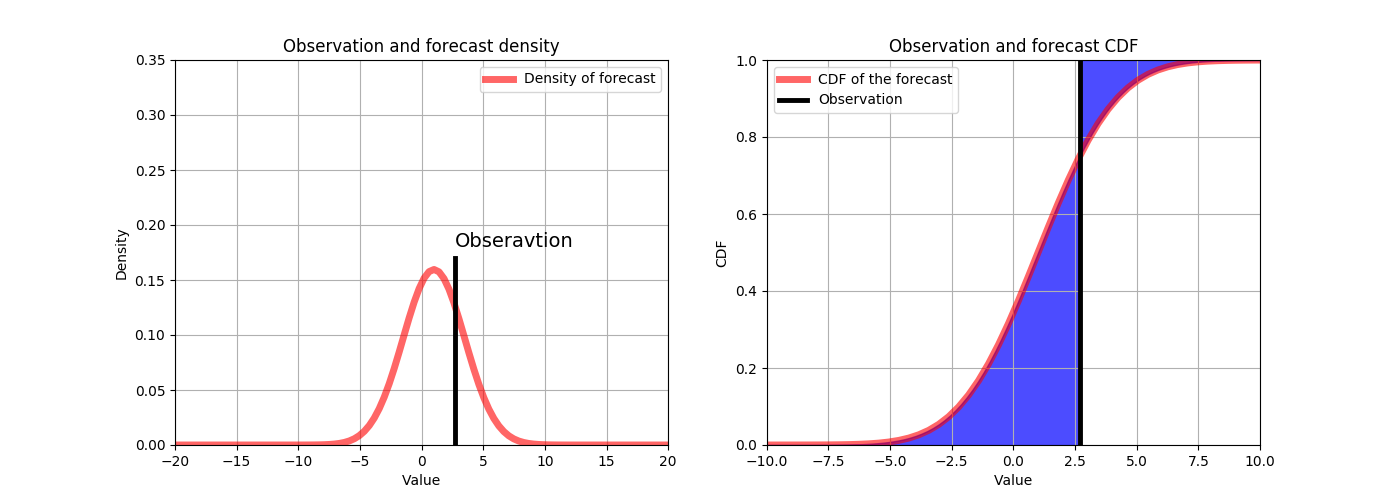
\includegraphics[height=0.5\textwidth, width=1\textwidth]{figures/crps.png}
    \caption[Continuous Rank Probability Score Intuition]{The square of the blue area is the value of the CRPS. Notice how if the predicted CDF were a step function (the case when the prediction is deterministic point estimate), the CRPS will be nothing more than the squared differnece between the observation and the prediction.}
  \end{figure}
\end{center}

\subsubsection{Dawid–Sebastiani score (DSS)}
\label{sec:dss}

For complex distributions even the CRPS can be hard to evaluated as it requires some estimate of the integral in \refeq{eq:crps}. The \emph{Dawid–Sebastiani score} (\emph{DSS}), introduced in \cite{dawid1999}, relies only on the first two central moments of a given predicted forecast \(F\). DSS is defined as
\begin{equation}
  DSS(F,y) =  \frac{(y-\mu_F)^2}{\sigma_F^2}+2\log(\sigma_F)
\end{equation}
Of the three rules the DSS is most simple to calculate as it requires only two simple metrics of the forecast. The only thing we need is the ability to draw samples from the distribution of the forecast and we could estimate the mean and variance.
\subsubsection{Computation of scoring rules}
\label{sec:eval-rules}

In this thesis we deal with sets of data and we need to evaluate the scoring rules on certain number of data points - on the test or train set. For this we take the average over the scores of all examples in a set. Let \(\{x_n, y_n\}_{n=1}^N\) be our set of interest and some model have generated set of forecasts \(\{F_n\}_{n=1}^N\) where forecast \(F_i\) is based on the features \(x_i\) and tries to predict the observation \(y_i\). The overall score \(\bar{S_N}\) of the scoring rule \(S\) then is
\begin{equation}
  S_N = \frac{1}{N}\sum_{i=1}^N S(F_i, y_i) \,
\end{equation}
This is the final metric on which we compare several probability models.

When it comes to calculating the rules themselves on concrete observations there are explicit forms for the three rules if the predicted forecast is normal distribution. Those are given in \reftab{tab:rules-table} and taken from \cite{gneiting2014}.

\begin{center}
  \renewcommand{\arraystretch}{1.7}
  \label{tab:rules-table}
  \begin{tabular}{|l|l|}
    \hline
    \setlength\extrarowheight{5cm}
    Scoring rule \(S\) & \(S(\mathcal{N}(\mu, \sigma^2), y)\)\\
    \specialrule{.15em}{.05em}{.05em} %\hline
    \setlength\extrarowheight{5cm}
    Logarithmic score & \(\frac{(y-\mu)^2}{2\sigma^2} + \log(\sigma) + \frac{1}{2}\log(2\pi)\)\\
    \hline
    \setlength\extrarowheight{5cm}
    Continuous ranked probability score & \(\sigma(\frac{y-\mu}{\sigma}(2\Phi(\frac{y-\mu}{\sigma}) -1)\)\\
                       & \(\quad\quad + 2\phi(\frac{y-\mu}{\sigma}) - \frac{1}{\pi})\)\\
    \hline
    Dawid–Sebastiani score & \(\frac{(y-\mu)^2}{\sigma^2}+2\log(\sigma)\)\\
    \hline
  \end{tabular}
  \captionof{table}{Closed forms of the scoring rules for normal distribution}
 \end{center}

All of the examined model in the thesis can generate samples from their predicted forecasts. The DSS can thus be trivially calculated just through the empirical mean and variance of the generated samples. The predicted density function of the MDN is a sum of density functions of the mixture components (see \refsec{sec:mdn}) so it can easily be evaluated with the LS. For the BNN we use density estimation methods described in \cite{silverman1986} and \cite{scott2015} to calculate the LS. Empirical CDFs are trivially computable with sample data. For sample set \(\{x_i\}_i=1^n\) the empirical CDF is
\begin{align}
  &\bar{F_n}(t)=\frac{1}{n}\sum_{i=1}^n1_{x_i\leq t} \\
  &\text{wehre} \\
  &1_{a\leq t} =
        \begin{cases}
          1 &,\text{if}\, a \leq t \\
          0 &,\text{if}\, a > t 
        \end{cases}
\end{align}
With this function we can also calculate the CRPS in straightforward manner following the definition in \refeq{eq:crps}.
% With that we've covered all cases in the evaluation of our models.
\subsection{Rank Histogram}
\label{sec:rank-hist}

\emph{Rank histograms} (sometimes called \emph{verification rank histogram}) are a tool for evaluating ensemble forecasts (\cite{hamill2001}). In our work however we adapt them to evaluate forecasts in form of probability distributions. The underlying assumption is that the ensemble member forecasts are distributed so as to delineate ranges. Let \([y_1^p,..., y_M^p]\) be a \emph{sorted} ensemble where each \(y_i^p\) is a predicted value for the true observation \(y^t\). The rank of \(y^t\) according to the ensemble is an integer \(k\) such that
\begin{equation}  
  rank(y^t)=
  \begin{cases}
    0,   & \text{if}\  y^t < y_1^p \\
    k,   & \text{if}\  y_{k}^p \leq y^t < y_{k+1}^p  \\
    k+1, & \text{if}\  y_{k+1}^p <  y^t  \\
  \end{cases}
\end{equation}
In our case the sorted ensemble is just a sorted sequence of drawn samples from the distribution predicted by the given model. We calculated the rank of each observation and then create a histogram with certain number of bins. To be noted is that the number of bins is considerably less than the number of samples. The amount of samples drawn from each model for each observation is in the order of tens of thousand while the number of bins for the rank histogram is no more than 20.

For a well calibrated forecast, the rank histogram should be uniform. U-shaped histograms indicate underdispersed predictive distributions, whereas hump or inverse-U-shaped histograms correspond to overdispersed predictive distributions (\cite{gneiting2014}, \cite{diebold1998}, \cite{hamill2001}). If the histogram is uniform we can say that the observation behaves as a sample from the forecast. This is essentially what a good forecast should exhibit. \reffig{fig:rank-hist} illustrates the said about rank histograms.

\phantomsection
\begin{center}
  \begin{figure}[htbp]
    \label{fig:rank-hist}
    \centering
    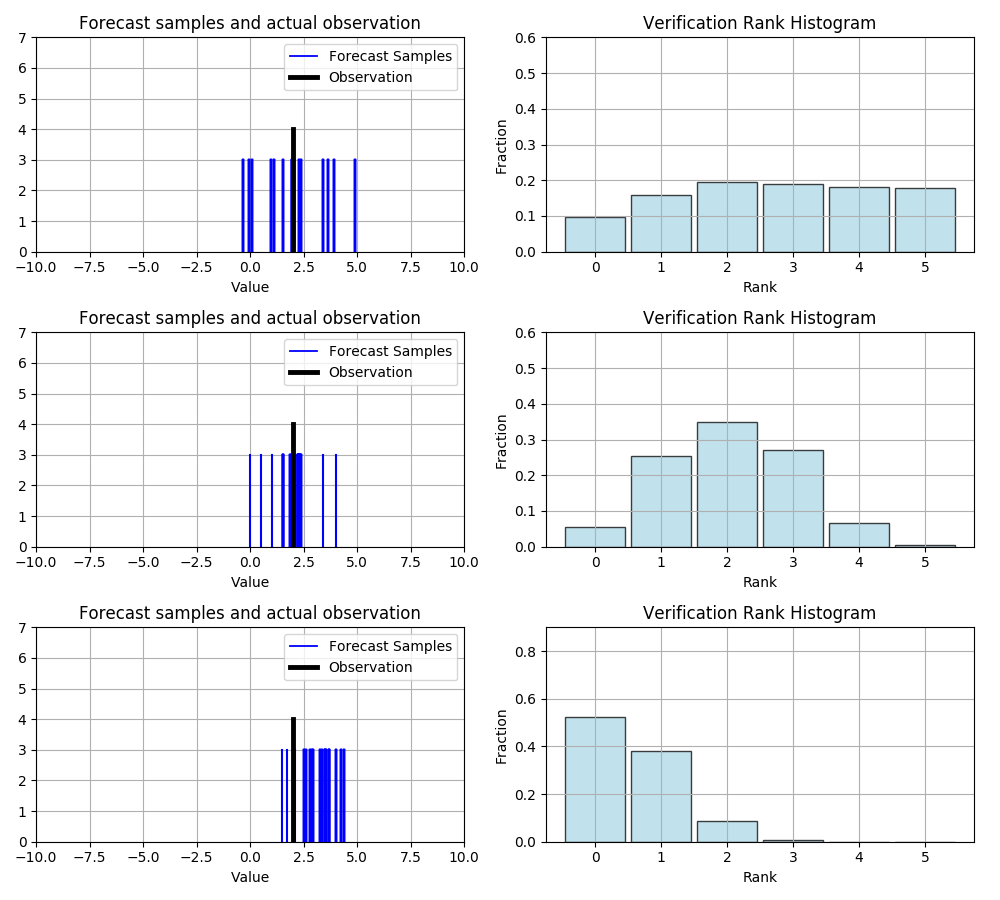
\includegraphics[height=0.75\textwidth, width=0.9\textwidth]{figures/verification_histogram.png}
    \caption[Rank Histogram Example]{Histograms illustrating different types of distributions with respect to the actual observations. To note is that on left we give only one example of samples drawn form the distribution in respect to a given observation. We assume that the sample sets for the other observations are similar and that this will produce the respective histograms on the right. A rank histogram cannot be given for a single observation and a single set of drawn samples.}
  \end{figure}
\end{center}
\subsection{Feature Importance}
\label{sec:feature-importance}

In order to asses the relative importance of the features used by the build models we use a method called \emph{permutation importance}. It is first described in  \cite{breiman2001} and it was applied to random forests. The techniques is also successfully applied in assessing the feature importance of ensemble methods for forecasting (\cite{lerch2018}). We closely follow the approach of \cite{lerch2018} by randomly shuffling each feature in the test and training sets and then look at the mean value of a given scoring rule. For each feature we examine the difference in the mean value of the scoring rules between the permuted and regular datasets.

We give formal definition of the described above. We consider a set of data \(\{x_n, y_n\}_{n=1}^N\) with feature vectors \(x_n\in\mathbb{R}^M\) and realized values \(y_n\in\mathbb{R}\). We define a matrix \(X\) with the features of all examples as
\begin{align}
  X &= \begin{bmatrix}
    x_{1} \\
    x_{2} \\
    \vdots \\
    x_{N}
  \end{bmatrix}
\end{align}
In this notation, the \(i^{th}\) row of the matrix are all of the features of the \(i^{th}\) example and the \(i^{th}\) column of the matrix are all of the \(i^{th}\) features of all examples. We further define \(F|x\) as the conditional forecast distribution given a vector of features of a input data point. We assume that \(F|x\) is predicted by some model. In essence we evaluate the importance of the used feature only in the context of the considered model. In this sense we examine which of the features have higher information value for the predictions of the given model.


Now we give formal definition for the permutation of the features. Let \(X_s\) denote the \(s^{th}\) column of the input data \(X\). Then the permuted set \(X^{\text{perm}_{\text{j}}}\) for the \(j^{th}\) feature is given by

\begin{equation}
  X^{\text{perm}_{\text{j}}} = 
  \begin{cases}
    X_{s},        & \text{if}\  j \neq s \\
    \pi(X_{(s)}), & \text{if}\  j = s
  \end{cases}
\end{equation}
where \(p(x)\) is some random permutation of the elements of the vector \(x\). Now we can give definition for the quantity that we call feature importance.
\begin{equation}
  \textit{Importance}(j) = \frac{1}{N}\sum_{n=1}^N (SR(F|X^{perm_j,(n)}, y_n) - SR(F|X^{(n)}, y_n) )
\end{equation}
where X\(^{\text{(n)}}\) is the feature vector of the \(n^{th}\) datapoint (i.e.\ the \(n^{th}\) row of the matrix \(X\)) and SR is some scoring rule - CRPS, DSS or LS in our case.

\section{Results}
\label{sec:res}
\subsection{Data used}
\label{sec:preprop-data} 
\subsection{Evaluation of the models}
\label{sec:eval-model}



\section{Implementation}
\label{sec:impl}
In order to enforce separation between the code and all of the data that the code act upon, we place all of the generated data in the \texttt{env} directory of the project. This directory is added to the \texttt{.gitignore} file so it the implantation in no way relies on it. The contents of the folder are fully generated with the execution of the implemented scripts. In the next section we explain exactly what is the generated content.
\subsection{Preparing the data}
\label{sec:prep-data}
In \refsec{sec:data} we mentioned that the public data that we use is less than ideal. We've also outline some of the problems that we found in the data. Now we like to explain how we deal with these problems. We've written several python scripts dealing with the prepossessing of the data. 

The raw data files are located under \cite{datalink}. They are organized in folders by day. The folder for a forgiven day contains different files from different sensor types. We are only interested in the air pollution data form the sds011 sensors. Each data file for this type of sensor is a text file with \emph{comma separated values} (\emph{CSV}) where each row has measurements for PM2.5 and PM10 (see \refsec{sec:data}), the location of the sensor, the time of day when the measurement was taken as well as the sensor id. Our final goal in the data preprocessing in to generate a DataFrame where each column is labeled with sensor id and either P1 (for PM2.5) or P2 (for PM10) and each row contains measurements of the corresponding integrated values for a certain period of time. The periods of time in which we integrate of course must be synchronized. In end effect we generate three different DataFrames from the data - with integration over whole days, over twelve hours and over one hour time periods.

We try to automate everything from downloading the data, extracting the relevant pieces of it, sanitizing it and finally generating a single \emph{DataFrame} object of \emph{pandas} (\cite{pandas}). As data prepossessing is not the focus of this thesis we don't explain each script in absolute detail but rather explain what happens in it.

All of the scripts we explain in this section require a configuration file. This file is \texttt{config.json}. In it we set certain properties for the scripts so that we could easily change them if necessary. In each of the scripts there is a \texttt{\_read\_config} method that loads the relevant for the script properties from the configuration file.
\subsubsection{Download module}
\label{sec:down-module}
The  amount of files under \cite{datalink}  is too big for the files to be downloaded manually. Therefore the first step of the process was to write a script that downloads the relevant files. This is the functionality provided by the \texttt{download\_module.py} file. In the configuration file there is a section with properties specifically for this script. Through those we can specify:
\begin{itemize}
\item \texttt{base\_url} - the base link where the files are located. In our case \url{https://archive.luftdaten.info/}
\item \texttt{start\_date}, \texttt{end\_date} - those specify the considered period of time. Only data files from this period will be downloaded. We've download files for the whole year of 2017.
\item \texttt{sensor\_type} - this fields specifies the type of information we want to download. We are dealing with air pollution and the considered sensor type is sds011 (see \refsec{sec:data}).
\item \texttt{files\_list\_file} - optional field specifying a file where the links and filenames of all downloaded files can be saved
\item \texttt{list\_files} - a boolean value showing weather or not the script should save the links of the downloaded files as a list in the file given in \texttt{files\_list\_file}
\end{itemize}
The script downloads the desired files in the directory given by the \texttt{raw\_down\_dir} property of the configuration file. Internally the script uses python bindings for \emph{wget} (\cite{wget}) in order to preform the actual downloading from the Internet. Another library that comes into use is \emph{BeautifulSoup} (\cite{bs}). With it we parse the \emph{HTML} of the web pages and extract \emph{desired} the URLs.

\subsubsection{Preprocess module}
\label{sec:preproc-module}
Central part of the preprocessing pipeline is the script in the \texttt{preprocess\_module.py} file. It aims to select only the data files from the ``good'' sensors, from those then further filter the data and then for each sensor that is reliable enough, to create a DataFrame in form of a CSV-file. The final CSV-files will be stored in the directory specified by the \texttt{data\_files\_dir} property in the configuration file. The \texttt{preprocess\_module} script first generates a file with the ids of the sensors that are actually worth processing. In this first phase we perform two checks while iterating over all of the downloaded files:
\begin{itemize}
\item For how many days a given sensor provides measurements. If a certain threshold is passed (given by the \texttt{min\_sensor\_cnt} property in the configuration), the sensors is considered as \emph{saturated}..
\item Is a given sensor ``around'' Stuttgart. In the configuration file we specify we specify a center (property \texttt{center}) and a radius (property \texttt{radius}) and consider sensors only in the defined circle.
\end{itemize}
If a given sensors passes both of those checks, its name is added to the file specified by the \texttt{good\_sensors\_list\_file} property. Furthermore, every data file of these ``good'' sensors is added to a file specified by the \texttt{good\_sensors\_data\_files\_list} property so that later we can process only those. 

The next step is to process the individual raw files and store their information in proper form in CSV-files. In this prepossessing for each file we do:
\begin{itemize}
\item We load the raw data file in memory in form of a pandas DataFrame.
\item We transform the time column in more convenient format and then perform check if there are any duplicates in the DataFrame with respect to the time of the measurement. If there are, we collapse them to a single entry by the strategy specified by \texttt{duplicates\_resolution} in the configuration. This could be \emph{MEAN}, \emph{MEDIAN}, \emph{MAX} or \emph{MIN}.
\item We then perform the integration over the desired time period specified by \texttt{day\_integration\_period} in the configuration. To note is that we are still working of file per file basis and the processed DataFrames contain a day worth of measurements. For the biggest integration period here is a day.
\item We rename the columns of the DataFrame to reflect the id of the corresponding sensor. The columns with measurements are then named \texttt{P1\_<id>} or \texttt{P2\_<id>} respectively for the integrated value for PM2.5 or PM10.
\item Here we make one final check in this phase. After the values in the DataFrames have been integrated over specific time intervals, there are still can be missing values. If those count of those missing values is higher than \texttt{missing\_data\_cnt\_threshold} in the configuration, the name of the sensors is added to a list in the file specified by \texttt{bad\_missing\_data\_sensors} property. If the missing values are below the mentioned threshold, then the missing values are interpolated by the strategy given by \texttt{missing\_data\_resolution} property. This could either be \emph{MEAN} (the missing values are filled with the average of the rest of the values) or \emph{linear} (the missing values are linearly interpolated based on the rest of the data).
\item After all of that we append the data of the resulting DataFrame to a CSV-file with name \texttt{end\_data\_frame\_<id>} in the direcotry specified by \texttt{data\_files\_dir}.
\end{itemize}
We do this for every raw data file and at the end we have a CSV-file for each sensor with accumulated data from the DataFrames. The final step is to go over these files one more time and sort the data by time.

\subsubsection{Description module}
\label{sec:desc-module}
The goal of this script is to provide some information about the generated data in from of plots and several DataFrames with statistics as well as to perform one final sanitation on the data. The script is implemented in the file \texttt{description\_module.py}. It iterates over the generated from the previous step DataFrames and counts the missing values. Its important that in this step the missing values are in the context of the whole year we are considering. Depending on the integration intervals there must be exactly certain amount of values in each DataFrame. For integration over a day the exact count is 356, for integration over 12 hours - 730, for integration over each hour of the year - 8760 (365 days time 24 hours per day). If the number of missing values in the corresponding context are grater than the value of the \texttt{missing\_entries\_threshold} property then the name of the sensor is added to a list in the file specified by \texttt{reindexed\_frames\_file}. If, however, the amount of missing values is under this threshold, the missing values are filled with the average value of the rest of the data. This is done of course both for the \texttt{P1} and \texttt{P2} column. As this is also our data description script, we generate a DataFrame with different statistics about the P1 and P2 values for each sensor. We wanted to know exactly how this last sanitation check on the data changes it so the DataFrames with the statistics are generated two times - once before the filling of the missing values and one time after the fact. We can then compare exactly what has changed about the data. At the end the scripts also generates plots of the P1 and P2 values of each sensor. Two kinds of plots are generated. One with the pure values as they appear in the final DataFrame. The other plot shows a moving average of 100 consecutive values. All of those description files are saved in the directory specified by the \texttt{description\_files\_dir} property in the configuration.

\subsubsection{Preprocess LU BW}
\label{sec:preproc-lu-bw-module}
Although the data provided from LU-BW is in much better form than the publicly available data, it also needs certain preprocessing. The LU-BW comes in form of several spreadsheets in form of a  \emph{xlsx} file. The script in \texttt{process\_lu\_bw.py} takes this file as an input and generates three DataFrames for each LU-BW station. The measurements in the spreadsheets are in half an hour basis so an integration in the desired intervals is required. The script performs this integration and fills all of the missing values with the mean of the rest of the data. Similar to the previous section, a description file with statistics about the data before and after the missing values filling is generated as well as plots with the integrated values and a moving average of them. The DataFrames are saved in CSV-files in a separate folder in the folder with the rest of the data files. The plots and the description file are saved in the directory with the description files. 

\subsubsection{Loader module}
\label{sec:load-module}
The final step is to put the individual DataFrames of the sensors in one big DataFrame that can be conveniently used for the training of the models. This is what the script in \texttt{loader\_module.py} performs. It gathers all the DataFrames defined by the CSV-files in the folder given by \texttt{folder} property and appends their columns to the columns to the final big DataFrame. The LU-BW DataFrames are also loaded. The final DataFrame is saved in the main \texttt{env} directory with name specified by \texttt{final\_df\_name}. In the section for this script of the configuration file there is a property with name \texttt{ignored\_sensors\_files}. This is meant to be a list of files, each containing a list of sensor ids. The sensors given in those files will be ignored and won't be loaded in the final DataFrame.


\subsection{Models implementations}
\label{sec:impl-model}
\noindent\emph{In the first two sections we explain the classes we've implemented for the two considered models. In the next two sections we describe the scripts that we use for training and evaluating the models.}
The major libraries we use are build on top of Tensorflow (\cite{tf}). In our explanations we assume basic knowledge of the principles and structures behind Tensorflow. A good introduction can be found in \cite{tfnintro}.
\subsubsection{Mixture density networks}
\label{sec:impl-mdn}
For the implementation of the MDNs we follow the guidance of \cite{mdntut}. We use the \emph{GPFlow} (\cite{gpflow}) library that internally uses Tensorflow. The library simplifies the creation of Gaussian process models. Although we don't unitize it fully, the features it provides make it really easy to define MDN.

The code implementing the MDN is in the \texttt{mdn\_model.py} file. In it we define a class - \texttt{Mdn} - representing a mixture density network. As previously stated, we follow the approach of \cite{mdntut}. Our \texttt{Mdn} class inherits from the \texttt{Model} class in the \texttt{gpflow.models.model} package. This base class makes it possible to integrate our newly defined model in the GPFlow library and later trained. In order to explain the structure and the functionality of our class we take a bottom-up approach. We first describe the individual small parts and then how they come together.

In the constructor of the class we define the basic attributes of the models that we'll need in the other functions. For the construction of and Mdn-object we need:
\begin{itemize}
\item An arbitrary name for the new model in form of a string in the argument \texttt{model\_id}
\item The training data for the model - \texttt{X} are the input feature vectors (as explained in \refsec{sec:feature-importance})  and \texttt{Y} is the output.
\item The definitions of the inner layers of the network. This is nothing more than an array of numbers specifying how many neurons there are each of the hidden layers. The number of hidden layers is given by the length of this array. In the constructor this is the \texttt{inner\_dims} argument.
\item Activation function that will be used as non-linearity in the neural network (see \refsec{sec:nn}), by default this is the \(\tanh\) function. This is given through the argument \texttt{activation}.
\item The number of mixture components that the MDN will model. As simple integer value in the \texttt{num\_mixtures} argument with default value of \(5\).
\item Optional file name of a file from which the class is supposed to load the model.
\end{itemize}
In the constructor itself we save the provided information in class attributes. Some of the more interesting ones are:
\begin{itemize}
\item \texttt{dims} - a two dimensional array that for each layers contains the dimensions of its input and output data. This makes it easier later to define the network in straight forward manner. To note is how the output dimension of the last layer is defined as in \refeq{eq:nn-ouput}.
\end{itemize}
After defining everything we either load the model (discussed later) from a file or construct it with the \texttt{\_create\_network} method.

The \texttt{\_create\_network} does nothing more than defining the weight matrices and bias vectors. The appropriate dimensions are known thanks to the \texttt{dims} array. The weight matrices are assigned random values and we expose restriction on the bias vectors to be positive in order introduce some regularization on the network (suggested by \cite{mdntut}, see \cite{hinz18}). All of the network's parameters are in the form of \texttt{Param} objects from GPFlow. Those encapsulate raw vector variables from Tensorflow that later could be learned and are managed by GPFlow. The generated parameters are put into class attributes for later use.

With the weights and biases defined we can describe the \texttt{\_eval\_network} method. In it we iterate over the weight matrices and biases and construct a Tensorflow graph defining the cascade of matrix multiplication, bias addition, non-linear function application as described in \refsec{sec:nn}. The method takes one input argument that is the input to the network. At the end of the matrix multiplications, we split the intermediate output in three parts - mixing coefficients, means and variances. We place the described in \refsec{sec:mdn} restrictions on them with the \texttt{softmax} and \texttt{exp} functions of Tensorflow. The end result of the method is a Tensorflow operation that when evaluated with some produces the output of the whole MDN as described in \refsec{sec:mdn}. To note is that the \texttt{\_eval\_network} is decorated with the \texttt{@params\_as\_tensors} decorator which transforms the arguments of the method as tensors automatically on invocation of the method.

The \texttt{\_eval\_network} method is used by \texttt{eval\_network} to actually provide output of the MDN to a user. \texttt{eval\_network} is defined with \texttt{@autoflow} decorator which automatically evaluates the returned tensorflow operations.

The most important method to be implemented so that GPFlow can train the model is \texttt{\_build\_likelihood}. It essentially defines the loss function to be optimized. In the method we first evaluate the network with the given input in order to generate the mixing coefficients, means and variances. Next we use these in order to build the sum over the log-likelihood over each example as described in \refsec{sec:mdn} and given in \refeq{eq:log-like-sum-1} and \refeq{eq:log-like-sum-2}. This is essentially all what we need to do as the automatic differentiation engine of Tensorflow does the gradient calculation. 

The \texttt{fit} method is the place where we do the actual training of the model. We use the \texttt{ScipyOptimizer} class provided by GPFlow as a wrapper of \emph{scipy} (\cite{scipy}) function for optimizing functions that uses the LM-BFGS method (see \refsec{sec:nn}). The fit method takes the maximum number of iterations and a optional callback function. We perform the training in three steps. First we optimize the function while we allow changes only in the weight matrices, then we optimize only by changing the bias vectors and finally we optimize with changes in both of the parameter groups. This is done to introduce a little bit more regularization in the training of the network. After each step we invoke the callback if provided, so that the outside user can monitor the changes in network's performance after each step.

We've also implemented a \texttt{save} method that can make a trained model persistent by saving in storage memory. The method uses a \texttt{Saver} object provided by GPFlow that can serialize parameters and parameter lists. In order to fully reconstruct the model later we only need the weight matrices and bias vectors. For this reason those are the only objects that we serialize and save.

The later loading of a given model is done through the \texttt{load} method. Its purpose is to load the weight matrices and bias vectors from a given file through the deserialization provided by the same \texttt{Saver} object use for saving. The \texttt{load} method essentially does the same thing as the \texttt{\_create\_network} method, it's just that now we load the objects from a file. The load method is in fact invoked instead of \texttt{\_create\_network} by the constructor if a file name is provided.
\subsubsection{Bayesian neural networks}
\label{sec:impl-bnn}
With the implementation of BNNs we again don't reinvent the wheel and use the \emph{Edward} (\cite{edward}) library. Edward is another library built on top of Tensorflow and it provides a lot of functionality that makes Bayesian learning easier to implement. We follow the official guide (\cite{bnntut}) to BNNs from the authors of Edward. The class implementing BNNs is Bnn and is located in the \texttt{bnn\_model.py}. We now look at the individual functions of our class in order to explain it.

The construction is trivial as the only thing it does is save the given name of the model in an class attribute.

First we'll look at the methods \texttt{generate\_prior\_vars} and \texttt{generate\_latent\_vars}. These methods are very similar. For given input and output dimensions for the whole network and layer definitions (analogous to \refsec{sec:impl-mdn}) they both define weight matrices and bias vectors as Normal distributions (i.e.\ we can later sample wight matrices and bias vectors from the defines objects) with the appropriate dimensions. The difference between the methods is the context in which they define the distributions. \texttt{generate\_prior\_vars} defines the prior distributions over the wights and biases. These are all standard normal distributions and correspond to the \(p\) distributions in \refsec{sec:var-inference}. \texttt{generate\_latent\_vars} defines distributions with trainable Tensorflow variables that later will be optimized. These distributions build the variational distribution (see \refsec{sec:var-inference}) that we will perform inference and will try to approach the posterior. The individual variational variables are assigned random value at the start. 

The \texttt{\_neural\_network} method does essentially the same thing as the \texttt{\_eval\_network} from the Mdn class. For a given input and two lists of weight matrices and bias vectors it creates an Tensorflow operation that evaluates to the output of the network defined by the weights and biases and with an input the given input. The non-linearity function that we use is \texttt{tanh}. 

With all these methods explained we can now look at the central part of the Bnn class. The \texttt{build} method is what builds the whole Tensorflow graph for the structure of the BNN and the operations we will need for the inference. First, with the usage of \texttt{generate\_prior\_vars} and \texttt{generate\_latent\_vars}, we generate the prior and latent distributions we will need for the network. Then we define a tensor placeholder for the input data, operation that defines a normal distribution centered at the network's output and small variance (see \refsec{sec:bayesian-inference}) and a placeholder for the actual observed output data. To note is that here we use the prior distributions while we define the network operation. The next step is to define the operation necessary for the evaluation of the BNN with new data. For that we define two placeholders - one for the input with which we want to evaluate the trained network and one for the number of samples we want to draw from the posterior distribution (i.e.\ how many network functions we will generate and evaluate, see \refsec{sec:nn-in-bayesian}). After the placeholders will define operation that evaluates to a stacked evaluations of networks defined with draws from the latent variables defining the variational distribution. To note is that we evaluate each network on the whole input. The final shape of the output of this operation will be  \(N \times s\) where \(N\) is the count of provided examples to evaluate and \(s\) is the number of samples we are supposed to draw from the BNN. The final thing in the \texttt{build} method is to initialize all the variables in the Tensorflow graph with execution of initialization operation and define a \texttt{Saver} object so that later we can save the trained model to storage memory.

The training of the model happens in the \texttt{fit} method. In it the Bayesian inference functionality of Edward comes into play. We first define a dictionary the represents a mapping between prior variable and its variational counterpart. This is the format that Edward requires. After that come some calculation necessary for implementing batching over the data. We then define the type of inference we will use for training the model. In our case, Kullback-Leibler divergence (see \refsec{sec:var-inference}). Edward provides convenient interface for this definition through the class \texttt{ed.KLqp}. Once the inference is defined and initialized we create three in one another loops over the data. We feed certain amount of examples to the \texttt{update} method. As we operate on batches of data, we can also present given batch several times in a row to the \texttt{update} method. This is the job of the inner most loop. The middle loop iterates over all the batches. The outermost loop counts the epochs. One Epoch is when the entire dataset is passed through the inference algorithm once. One thing to note is that every one thousand epochs we invoke a callback if given. This way the outside user can monitor the models during the inference process.

With the \texttt{evaluate} methods we can evaluate data with some trained model. The method accepts the input data and samples to be drawn for each data point, feeds them to the write placeholders in the graph and evaluates the Tensorflow operation.

The \texttt{save} and \texttt{load} methods of the class are similar to the ones in the Mdn class. One key difference is that here we use the \texttt{Saver} object from Tensorflow and not from GPFlow. This means that by serialization we are saving the whole Tensorflow graph and the values of all variables in it. By the loading of the model later, we only need to load the graph and not build anything at all (i.e.\ not call the \texttt{build} method). 
\subsection{Model training}
\label{sec:models-train}
\subsection{Models evaluation}
\label{sec:models-eval}

\subsection{Auxiliary scripts}
\label{sec:aux-scripts}
\noindent\emph{Bash script that are aimed at automating some of the trivial tasks.} 
\subsubsection{Run Generation pipeline}
\label{sec:gen-pipe}
\noindent\emph{File:}\texttt{run\_generation\_pipeline.sh}

The script performs the whole DataFrame generation with the current \texttt{config.json} from start to finish. The steps that are automatically executed:
\begin{enumerate}
\item Extracts the integration period \texttt{P} for the data
\item Creates a log file with name \texttt{LOG\_<P>.txt} that will contain the whole output to the standard output of the scripts in the next steps.
\item Runs \texttt{preprocess\_module.py} with the right flags to generate cache files containing the senors that must be preprocessed.
\item Runs \texttt{preprocess\_module.py} with the right flags to perform the actual preprocessing of the raw files.
\item Runs \texttt{preprocess\_lu\_bw.py} to preprocess the LU-BW data.
\item Runs \texttt{description\_module.py} to perform the final checks on the data and generate plots and statistics about it
\item Counts the lines in each of the generated CSV-files for the data form \emph{luftdaten.info}. All of these numbers must be the same if everything is ok.
\item Counts the lines in each of the generated CSV-files for the data form LU-BW. All of these numbers must be the same if everything is ok.
\item Runs \texttt{loader\_module.py} to generate the final big DataFrame with all of the data.
\item Copies the final DataFrame in the \texttt{data\_frames} folder of the \texttt{env} directory.
\item Archives all of the generated files during the whole process including the log file, the \texttt{config.json} file, all of the generated data files, all of the generated description files.
\end{enumerate}
The result of running this script is a self-contained archive containing the generated data as well as description of how it was generated. This archive can later be inspected in order to validate the correctness of the data. One can also examine the log file and the configuration file and know what has happened exactly in the generation process.

Some of the steps are placed in bash scripts of their own. These scripts are with self expiatory names and we don't go over details about them rather just mentiom them: \texttt{preprocess\_new\_cache.sh} (step 3.), \texttt{preprocess\_with\_cached.sh} (step 4.), \texttt{save\_final\_dfs.sh} (step 10.), \texttt{archive\_data\_files.sh} (step 11.).


\subsubsection{Clean \texttt{env}}
\label{sec:script-clean}
\noindent\emph{File:}\texttt{clean.sh}

The scripts deletes all files  generated during the generation process expect the final data frame and the created archive. This prepares the \texttt{env} directory for a future execution of the preprocess pipeline.


\section{Conclusion}
\label{sec:conclusion}
\subsection{Summery}
\subsection{Discussion}



% The text ends here
\clearpage
\bibliographystyle{alpha}
\bibliography{references}
\end{document}
